\chapter{Results}\label{cha:results}
This chapter presents the results of the project. The results are shown in the form of experiments. All experiments are based on the problem statement from \autoref{sec:problem-statement}. The experiments are presented in the following order:


\begin{enumerate}
    \item \textbf{Experiment 1:} How does the choice of dimensionality reduction methods impact the errors, runtime and F1 score of the pipeline, when used with the best hyperparameters?
    \item \textbf{Experiment 2:} How many dimensions can a method reduce before a significant loss of accuracy occurs?
    \item \textbf{Experiment 3:} What impact do kernels and hyperparameters have on the dimensionality reduction methods?
    \item \textbf{Experiment 4:} How does accuracy and training time change when using different amounts of data?
\end{enumerate}



\todo{Rewrite this standard thing}
The second experiment will be done on a subset of the entire dataset. With 15.000 samples in the training set and the usual 10.000 samples in the test set. Instead of the standard 60.000 samples in the training set and 10.000 in the test set. The smaller sample size is used due to memory constraints regarding the nonlinear methods, as they need more memory than was available.


\section{Experiment 1}\label{sec:experiment-1}
%Needs an introduction to the experiment, and why it is relevant to the problem statement.
% relevance to problem anal. and introduction (why is this relavant)
The problem statement states to find the impact of dimensionality reduction, comparing linear and nonlinear methods. This experiment compares the chosen dimensionality reduction methods in each of their best configurations on the chosen MNIST dataset. This experiment is relevant to the problem statement, as it is the first step in finding the impact of dimensionality reduction. The experiment is also relevant to the problem analysis, as it explores the impact of dimensionality reduction in ML. The experiment also finds the best configuration for each method was essential to comparing the methods on the same number of samples.



\subsection{Rules and overview of experiment}\label{subsec:experiment-1-rules}
% Rules and what have we done, how do we evaluate (write about specs here)
The dimensionality reduction methods used in the experiment were \gls{svm}, \gls{pca}, \gls{lda}, \gls{kpca}, and \gls{isomap}. The baseline SVM ML model was also used without any dimensionality reduction. Each method was first cross-validated, finding the best hyperparameters for 15000 samples. Every method was tested with the same number of components. Besides LDA, it can only use up to 9 components. Then some of the methods were cross-validated again with 60000 samples to find how the methods performed with more data; the same components were still used. The methods tested on 60000 samples were the baseline SVM, PCA, and LDA, as the computer used in the experiment could not handle kPCA and ISOMAP with 60000 samples of data. The configurations used for each are shown in Table \ref{tab:best-configuration}.

\begin{table}[htb!]   
    \centering
    \begin{tabular}{lrlll}
        \toprule
        method & components & C & parameter & parameter\\
        \midrule
        SVM-15 & 784 & C = 0.01 &  \\
        SVM-60 & 784 & C = 0.01 &  \\
        LDA-15 & 9 & C = 0.1 &  \\
        LDA-60 & 9 & C = 1.0 &  \\
        PCA-15 & 49 & C = 0.01 &  \\
        PCA-60 & 49 & C = 0.1 &   \\
        KPCA-15 & 49 & C = 1.0 & Gamma = 0.01 & Sigmoid \\
        ISOMAP-15 & 49 & C = 0.001 & neighbours = 5 \\
        \bottomrule
    \end{tabular}
    \caption{Best configuration for each method used for experiment-1, method-15 and method-60, means the method with 15 and 60 thousand samples.}
    \label{tab:best-configuration}
\end{table}

Every test in experiment 1 was made on the same computer, namely pc-2. See \autoref{tab:pc-specs} for the specific specs for the comuter used in the experiment. 

The experiment results are shown in \autoref{subsec:experiment-1-results}. The results are in the form of classification reports and confusion matrixes, which show the precision, recall, f1-score, support for each class, and the total accuracy for each method. The methods will be compared in accuracy, f1-score, and time fitting the data.

\subsection{Results}\label{subsec:experiment-1-results}
% Show results (desribe the most relavant results)
Below is shown the results for the methods. The results are in the form of classification reports, which show the precision, recall, f1-score, support for each class, and the total accuracy for each method. The methods will be compared in accuracy, f1-score, and time fitting the data. 

\begin{table}[htb!]
\centering
\begin{tabular}{lrrrr}
\toprule
 & precision & recall & f1-score & support \\
\midrule
0 & 94.7886 & 98.3673 & 96.5448 & 980 \\
1 & 96.3979 & 99.0308 & 97.6967 & 1135 \\
2 & 92.2488 & 93.4109 & 92.8262 & 1032 \\
3 & 90.8203 & 92.0792 & 91.4454 & 1010 \\
4 & 93.4739 & 94.8065 & 94.1355 & 982 \\
5 & 90.7940 & 88.4529 & 89.6082 & 892 \\
6 & 95.6705 & 94.5720 & 95.1181 & 958 \\
7 & 94.4828 & 93.2879 & 93.8815 & 1028 \\
8 & 93.1842 & 89.8357 & 91.4794 & 974 \\
9 & 92.8717 & 90.3865 & 91.6123 & 1009 \\
accuracy & & & 93.5400 & 10000 \\
macro avg & 93.4733 & 93.4230 & 93.4348 & 10000 \\
weighted avg & 93.5263 & 93.5400 & 93.5199 & 10000 \\
\bottomrule
\end{tabular}
\caption{Classification report for baseline\_svm\_15000}
\label{tab:classification-report-baseline_svm_15000}
\end{table}
 %37
\begin{figure}[htb!]
    \centering
    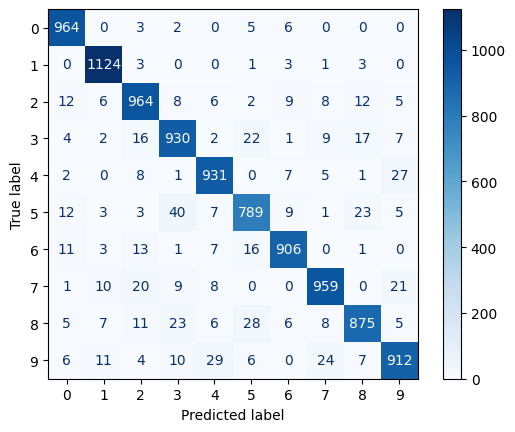
\includegraphics[width=0.8\textwidth]{figures/1-experiment/confusion_matrix_baseline_svm_15000.png}
    \caption{Confusion matrix for baseline SVM with 15000 samples.}
    \label{fig:confusion-matrix-baseline_svm_15000}
\end{figure}
\subsubsection{\gls{svm} with 15000 samples}\label{subsubsec:experiment-1-results-svm-15000}
Table \ref{tab:classification-report-baseline_svm_15000} shows the accuracy for \gls{svm} without any dimensionality reduction with 15000 samples. The accuracy is 93.54\%, and it takes 37 seconds to train the model. \autoref{fig:confusion-matrix-baseline_svm_15000} shows \gls{svm} is best at recognizing zeros and one's in pictures, as the model has the f1-score in these classes, with the scores 96.5\% and 97.7\%. The model has some trouble recognizing fives, eights, and threes, as these are the lowest scoring in the f1-score for all the classes, with five being 89.6\%, eight being 91.5\%, and three being 91.4\%. With an average f1-score of 93.43\%, the baseline \gls{svm} with 15000 samples is a good model. 

\subsubsection{\gls{svm} with 60000 samples}\label{subsubsec:experiment-1-results-svm-60000}
\begin{table}[htb!]
\centering
\begin{tabular}{lrrrr}
    \toprule
    & precision & recall & f1-score & support \\
    \midrule
    0 & 96.0278 & 98.6735 & 97.3327 & 980 \\
    1 & 97.3958 & 98.8546 & 98.1198 & 1135 \\
    2 & 93.6538 & 94.3798 & 94.0154 & 1032 \\
    3 & 91.6587 & 94.6535 & 93.1320 & 1010 \\
    4 & 93.8124 & 95.7230 & 94.7581 & 982 \\
    5 & 92.4138 & 90.1345 & 91.2599 & 892 \\
    6 & 96.2105 & 95.4071 & 95.8071 & 958 \\
    7 & 95.6262 & 93.5798 & 94.5919 & 1028 \\
    8 & 93.4668 & 91.0678 & 92.2517 & 974 \\
    9 & 94.8012 & 92.1705 & 93.4673 & 1009 \\
    accuracy & & & 94.5600 & 10000\\
    macro avg & 94.5067 & 94.4644 & 94.4736 & 10000 \\
    weighted avg & 94.5599 & 94.5600 & 94.5481 & 10000 \\
    \bottomrule
\end{tabular}
\caption{Classification report for baseline\_svm\_60000}
\label{tab:classification-report-baseline_svm_60000}
\end{table}
 %378
% \begin{figure}[htb!]
%     \centering
%     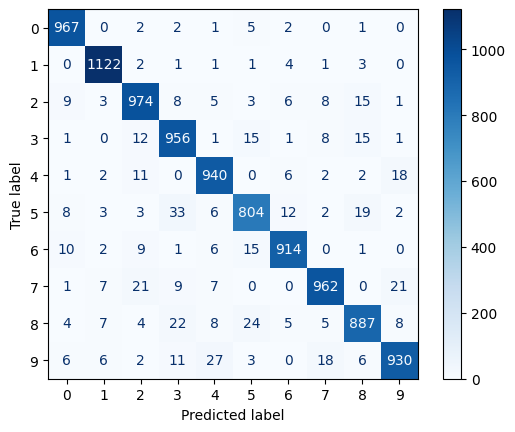
\includegraphics[width=0.8\textwidth]{figures/1-experiment/confusion_matrix_baseline_svm_60000.png}
%     \caption{Confusion matrix for baseline SVM with 60000 samples.}
%     \label{fig:confusion-matrix-baseline_svm_60000}
% \end{figure}
Table \ref{tab:classification-report-baseline_svm_60000} shows the accuracy for \gls{svm} without any dimensionality reduction with 60000 samples. The accuracy is 94.56\% for 60000 samples, and it takes 378 seconds to train the model, which is 6 minutes and 16 seconds. The \gls{svm} model is best at recognizing zeros and ones in pictures, as the model has the f1-score in these classes, with scores of 97.3\% and 98.1\%. The model has some trouble recognizing fives, eights, and threes, as these are the lowest scoring in the f1-score for all the classes, with five being 91.2\%, eight being 92.3\%, and three being 93.1\%. With an average f1-score of 94.47\%, the baseline \gls{svm} with 15000 samples is a good model that uses a significant amount of time.

\subsubsection{\gls{lda} with 15000 samples}\label{subsubsec:experiment-1-results-lda-15000}
\begin{table}[htb!]
\centering
\begin{tabular}{lrrrr}
    \toprule
    & precision & recall & f1-score & support \\
\midrule
0 & 93.1238 & 96.7347 & 94.8949 & 980 \\
1 & 94.3869 & 96.2996 & 95.3336 & 1135 \\
2 & 89.2246 & 85.8527 & 87.5062 & 1032 \\
3 & 85.1781 & 87.6238 & 86.3836 & 1010 \\
4 & 86.9650 & 91.0387 & 88.9552 & 982 \\
5 & 83.6549 & 82.6233 & 83.1359 & 892 \\
6 & 92.1466 & 91.8580 & 92.0021 & 958 \\
7 & 90.3353 & 89.1051 & 89.7160 & 1028 \\
8 & 83.2804 & 80.8008 & 82.0219 & 974 \\
9 & 87.7193 & 84.2418 & 85.9454 & 1009 \\
accuracy & & & 88.7600 & 10000 \\
macro avg & 88.6015 & 88.6178 & 88.5895 & 10000 \\
weighted avg & 88.7285 & 88.7600 & 88.7240 & 10000 \\
\bottomrule
\end{tabular}
\caption{Classification report for lda svm 15000}
\label{tab:classification-report-lda_svm_15000}
\end{table}
 %7
\begin{figure}[htb!]
    \centering
    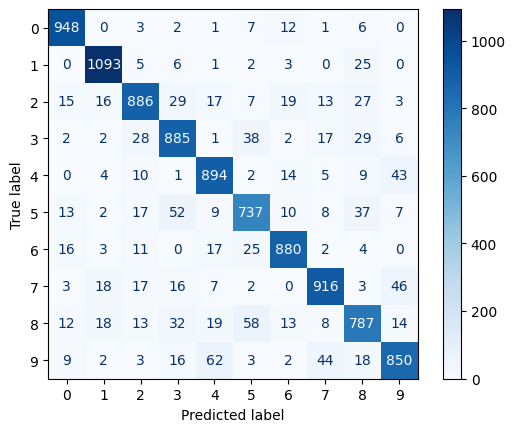
\includegraphics[width=0.8\textwidth]{figures/1-experiment/confusion_matrix_lda_svm_15000.png}
    \caption{Confusion matrix for LDA with 15000 samples.}
    \label{fig:confusion-matrix-lda-15000}
\end{figure}
Table \ref{tab:classification-report-lda_svm_15000} shows the accuracy for \gls{svm} with \gls{lda} as dimensionality reduction with 15000 samples. The accuracy is 88.76\% for 15000 samples, and it takes 7 seconds to train the model. \autoref{fig:confusion-matrix-lda-15000} \gls{svm} model is best at recognizing zeros and ones in pictures, as the model has the f1-score in these classes, with scores of 94.9\% and 95.3\%. The model has some trouble recognizing fives, eights, and nines, as these are the lowest scoring in the f1-score for all the classes, with five being 83.1\%, eight being 82.0\%, and three being 85.9\%. With an average f1-score of 88.59\%, the baseline \gls{svm}with 15000 samples is a worse model but is much faster than simply using \gls{svm}.
\subsubsection{\gls{lda} with 60000 samples}\label{subsubsec:experiment-1-results-lda-60000}
\begin{table}[htb!]
\centering
\begin{tabular}{lrrrr}
    \toprule
    & precision & recall & f1-score & support \\
    \midrule
0 & 93.1953 & 96.4286 & 94.7844 & 980 \\
1 & 94.7232 & 96.4758 & 95.5914 & 1135 \\
2 & 90.0398 & 87.5969 & 88.8016 & 1032 \\
3 & 85.9804 & 86.8317 & 86.4039 & 1010 \\
4 & 88.0929 & 92.6680 & 90.3226 & 982 \\
5 & 84.4318 & 83.2960 & 83.8600 & 892 \\
6 & 91.0387 & 93.3194 & 92.1649 & 958 \\
7 & 90.7093 & 88.3268 & 89.5022 & 1028 \\
8 & 84.9520 & 81.7248 & 83.3072 & 974 \\
9 & 88.4892 & 85.3320 & 86.8819 & 1009 \\
accuracy & & & 89.3300 & 10000 \\
macro avg & 89.1653 & 89.2000 & 89.1620 & 10000 \\
weighted avg & 89.2917 & 89.3300 & 89.2903 & 10000 \\
\bottomrule
\end{tabular}
\caption{Classification report for lda svm 60000}
\label{tab:classification-report-lda_svm_60000}
\end{table}
 %58
% \begin{figure}[htb!]
%     \centering
%     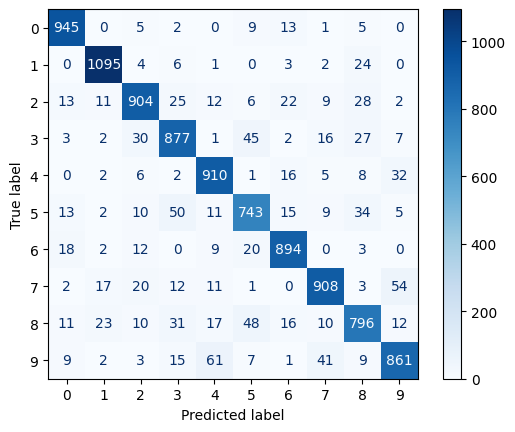
\includegraphics[width=0.8\textwidth]{figures/1-experiment/confusion_matrix_lda_svm_60000.png}
%     \caption{Confusion matrix for LDA with 60000 samples.}
%     \label{fig:confusion-matrix-lda-60000}
% \end{figure}
Table \ref{tab:classification-report-lda_svm_60000} shows the accuracy for \gls{svm} with \gls{lda} as dimensionality reduction with 60000 samples. The accuracy is 89.33\% for 60000 samples, and it takes 58 seconds to train the model. The \gls{svm} model is best at recognizing zeros and ones in pictures, as the model has the f1-score in these classes, with scores of 94.8\% and 95.6\%. The model has some trouble recognizing fives, eights, and threes, as these are the lowest scoring in the f1-score for all the classes, with five being 83.9\%, eight being 83.3\%, and three being 86.4\%. \gls{svm} using \gls{pca} as the dimensionality reduction method has an average f1-score of 89.16\%.

\subsubsection{\gls{pca} with 15000 samples}\label{subsubsec:experiment-1-results-pca-15000}
\begin{table}[htb!]
\centering
\caption{Classification report for pca_svm_15000}
\label{tab:classification-report-pca_svm_15000}
\begin{tabular}{lrrrr}
\toprule
 & precision & recall & f1-score & support \\
\midrule
0 & 0.944773 & 0.977551 & 0.960883 & 980.000000 \\
1 & 0.967938 & 0.984141 & 0.975972 & 1135.000000 \\
2 & 0.904306 & 0.915698 & 0.909966 & 1032.000000 \\
3 & 0.897335 & 0.900000 & 0.898665 & 1010.000000 \\
4 & 0.916914 & 0.943992 & 0.930256 & 982.000000 \\
5 & 0.889143 & 0.872197 & 0.880589 & 892.000000 \\
6 & 0.951832 & 0.948852 & 0.950340 & 958.000000 \\
7 & 0.923002 & 0.921206 & 0.922103 & 1028.000000 \\
8 & 0.904963 & 0.879877 & 0.892244 & 974.000000 \\
9 & 0.927083 & 0.882061 & 0.904012 & 1009.000000 \\
accuracy & 0.923700 & 0.923700 & 0.923700 & 0.923700 \\
macro avg & 0.922729 & 0.922558 & 0.922503 & 10000.000000 \\
weighted avg & 0.923513 & 0.923700 & 0.923467 & 10000.000000 \\
\bottomrule
\end{tabular}
\end{table}
 %10
\begin{figure}[htb!]
    \centering
    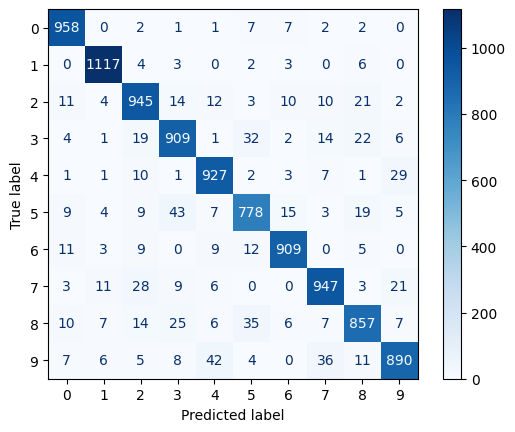
\includegraphics[width=0.8\textwidth]{figures/1-experiment/confusion_matrix_pca_svm_15000.png}
    \caption{Confusion matrix for PCA with 15000 samples.}
    \label{fig:confusion-matrix-pca-15000}
\end{figure}
Table \ref{tab:classification-report-pca_svm_15000} shows the accuracy for \gls{svm} with \gls{pca} as dimensionality reduction with 15000 samples. The accuracy is 92.37\% for 15000 samples, and it takes 10 seconds to train the model. \autoref{fig:confusion-matrix-pca-15000} \gls{svm} model is best at recognizing zeros and ones in pictures, as the model has the f1-score in these classes, with scores of 96.1\% and 97.6\%. The model has some trouble recognizing fives, eights, and threes, as these are the lowest scoring in the f1-score for all the classes, with five being 88.1\%, eight being 89.2\%, and three being 89.9\%. \gls{svm} using \gls{pca} as the dimensionality reduction method has an average f1-score of 92.25\%.

\subsubsection{\gls{pca} with 60000 samples}\label{subsubsec:experiment-1-results-pca-60000}
\begin{table}[htb!]
\centering
\begin{tabular}{lrrrr}
    \toprule
    & precision & recall & f1-score & support \\
    \midrule
    0 & 94.8768 & 98.2653 & 96.5414 & 980 \\
    1 & 96.7993 & 98.5903 & 97.6866 & 1135 \\
    2 & 92.3301 & 92.1512 & 92.2405 & 1032 \\
    3 & 88.9952 & 92.0792 & 90.5109 & 1010 \\
    4 & 92.3153 & 95.4175 & 93.8408 & 982 \\
    5 & 90.4157 & 87.7803 & 89.0785 & 892 \\
    6 & 95.7336 & 96.0334 & 95.8833 & 958 \\
    7 & 94.3620 & 92.8016 & 93.5753 & 1028 \\
    8 & 92.2340 & 89.0144 & 90.5956 & 974 \\
    9 & 93.7565 & 89.2963 & 91.4721 & 1009 \\
    accuracy &  & & 93.2500 & 10000\\
    macro avg & 93.1819 & 93.1429 & 93.1425 & 10000 \\
    weighted avg & 93.2474 & 93.2500 & 93.2290 & 10000 \\
\bottomrule
\end{tabular}
\caption{Classification report for pca svm 60000}
\label{tab:classification-report-pca_svm_60000}
\end{table}
 %97
% \begin{figure}[htb!]
%     \centering
%     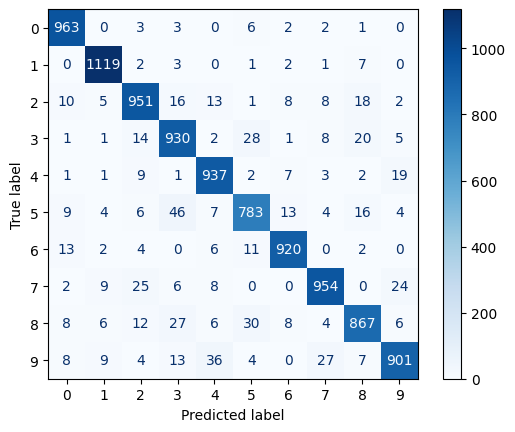
\includegraphics[width=0.8\textwidth]{figures/1-experiment/confusion_matrix_pca_svm_60000.png}
%     \caption{Confusion matrix for PCA with 60000 samples.}
%     \label{fig:confusion-matrix-pca-60000}
% \end{figure}
Table \ref{tab:classification-report-pca_svm_60000} shows the accuracy for \gls{svm} with \gls{pca} as dimensionality reduction with 60000 samples. The accuracy is 93.25\% for 60000 samples, and it takes 97 seconds to train the model, which is 1 minute and 37 seconds. The \gls{svm} model is best at recognizing zeros and ones in pictures, as the model has the f1-score in these classes, with scores of 96.5\% and 97.7\%. The model has some trouble recognizing fives, eights, and threes, as these are the lowest scoring in the f1-score for all the classes, with five being 89.1\%, eight being 90.6\%, and three being 90.5\%. \gls{svm} using \gls{pca} as the dimensionality reduction method has an average f1-score of 93.14\%.

\subsubsection{\gls{kpca} with 15000 samples}\label{subsubsec:experiment-1-results-kernel_pca-15000}
\begin{table}[htb!]
\centering
\caption{Classification report for kernel_pca_svm_15000}
\label{tab:classification-report-kernel_pca_svm_15000}
\begin{tabular}{lrrrr}
\toprule
 & precision & recall & f1-score & support \\
\midrule
0 & 0.943137 & 0.981633 & 0.962000 & 980.000000 \\
1 & 0.968858 & 0.986784 & 0.977739 & 1135.000000 \\
2 & 0.911005 & 0.922481 & 0.916707 & 1032.000000 \\
3 & 0.893175 & 0.894059 & 0.893617 & 1010.000000 \\
4 & 0.915842 & 0.941955 & 0.928715 & 982.000000 \\
5 & 0.881609 & 0.859865 & 0.870602 & 892.000000 \\
6 & 0.937824 & 0.944676 & 0.941238 & 958.000000 \\
7 & 0.929342 & 0.921206 & 0.925256 & 1028.000000 \\
8 & 0.927039 & 0.887064 & 0.906611 & 974.000000 \\
9 & 0.916667 & 0.883053 & 0.899546 & 1009.000000 \\
accuracy & 0.923600 & 0.923600 & 0.923600 & 0.923600 \\
macro avg & 0.922450 & 0.922278 & 0.922203 & 10000.000000 \\
weighted avg & 0.923360 & 0.923600 & 0.923321 & 10000.000000 \\
\bottomrule
\end{tabular}
\end{table}
 %92
\begin{figure}[htb!]
    \centering
    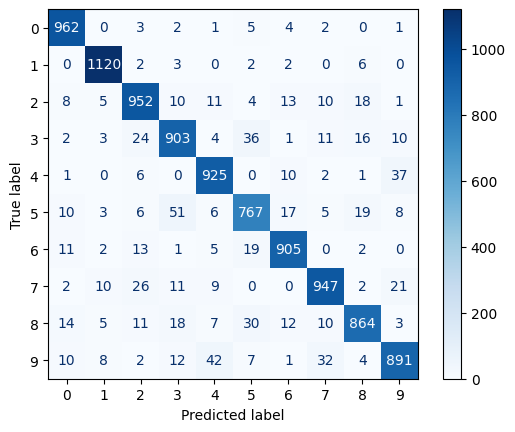
\includegraphics[width=0.8\textwidth]{figures/1-experiment/confusion_matrix_kernel_pca_svm_15000.png}
    \caption{Confusion matrix for kernel PCA with 15000 samples.}
    \label{fig:confusion-matrix-kpca-15000}
\end{figure}
Table \ref{tab:classification-report-kernel_pca_svm_15000} shows the accuracy for \gls{svm} with \gls{kpca} as dimensionality reduction with 15000 samples. The accuracy is 92.36\% for 15000 samples, and it takes 92 seconds to train the model, which is 1 minute and 32 seconds. \autoref{fig:confusion-matrix-kpca-15000} \gls{svm} model is best at recognizing zeros and ones in pictures, as the model has the f1-score in these classes, with scores of 96.2\% and 97.8\%. The model has trouble recognizing fives, nines, and threes, as these are the lowest scores in the f1-score for all the classes, with five being 87.1\%, nine being 90.0\%, and three being 89.4\%. \gls{svm} using \gls{kpca} as the dimensionality reduction method has an average f1-score of 92.22\%.

\subsubsection{\gls{isomap} with 15000 samples}\label{subsubsec:experiment-1-results-isomap-15000}
\begin{table}[htb!]
\centering
\begin{tabular}{lrrrr}
    \toprule
 & precision & recall & f1-score & support \\
\midrule
0 & 93.1507 & 97.1429 & 95.1049 & 980 \\
1 & 94.2953 & 99.0308 & 96.6051 & 1135 \\
2 & 92.1509 & 87.5969 & 89.8162 & 1032 \\
3 & 88.2579 & 90.7921 & 89.5071 & 1010 \\
4 & 91.5725 & 90.7332 & 91.1509 & 982 \\
5 & 87.7232 & 88.1166 & 87.9195 & 892 \\
6 & 95.1426 & 94.0501 & 94.5932 & 958 \\
7 & 88.5375 & 87.1595 & 87.8431 & 1028 \\
8 & 89.7297 & 85.2156 & 87.4144 & 974 \\
9 & 84.8963 & 85.2329 & 85.0643 & 1009 \\
accuracy & & & 90.6100 & 10000\\
macro avg & 90.5457 & 90.5071 & 90.5019 & 10000 \\
weighted avg & 90.5947 & 90.6100 & 90.5771 & 10000 \\
\bottomrule
\end{tabular}
\caption{Classification report for isomap\_svm\_15000}
\label{tab:classification-report-isomap_svm_15000}
\end{table}
 %165
\begin{figure}[htb!]
    \centering
    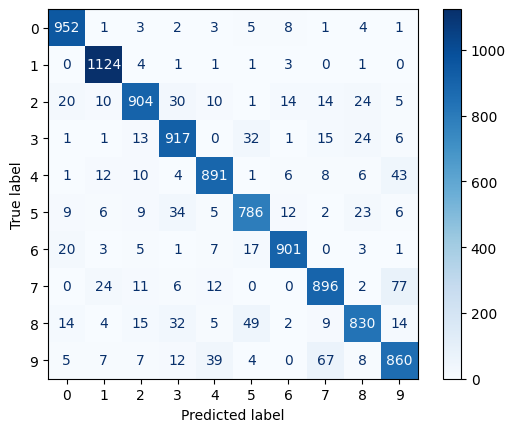
\includegraphics[width=0.8\textwidth]{figures/1-experiment/confusion_matrix_isomap_svm_15000.png}
    \caption{Confusion matrix for ISOMAP with 15000 samples.}
    \label{fig:confusion-matrix-isomap-15000}
\end{figure}
Table \ref{tab:classification-report-isomap_svm_15000} shows the accuracy for \gls{svm} with \gls{isomap} as dimensionality reduction with 15000 samples. The accuracy is 90.61\% for 15000 samples, and it takes 165 seconds to train the model, which is 2 minutes and 45 seconds. \autoref{fig:confusion-matrix-isomap-15000} \gls{svm} model is best at recognizing zeros and ones in pictures, as the model has the f1-score in these classes, with scores of 95.1\% and 96.6\%. The model has trouble recognizing sevens, eights, and nines, as these are the lowest scoring in the f1-score for all the classes, with seven being 87.8\%, eight being 87.4\%, and three being 85.1\%. \gls{svm} using \gls{isomap} as the dimensionality reduction method has an average f1-score of 90.50\%.

\subsection{Discussion experiment 1}\label{sec:discussion-experiment-1}
% discus the results to the problem statement
Comparing the results from experiment 1 is done in two comparisons; the first comparison is between the accuracy and time for the different dimensionality reduction methods. The second comparison is between the f1-scores for the different dimensionality reduction methods and what numbers the models are worst at recognizing. 

\subsubsection{Accuracy and time}\label{subsec:discussion-experiment-1-accuracy}
All experiments done is displayed in Table \ref{tab:discussion-experiment-1-accuracy}, it shows the accuracy for all the different models and the time taken.

\begin{table}
    \centering
    \begin{tabular}{lll}
        \hline
        Reduction method & Accuracy & Time \\
        \hline
        \gls{svm}-15 & 93.54\% & 37 seconds \\
        \gls{lda}-15 & 88.76\% & 7 seconds \\
        \gls{pca}-15 & 92.37\% & 10 seconds \\
        \gls{kpca}15 & 92.36\% & 92 seconds \\
        \gls{isomap}-15 & 90.61\% & 165 seconds \\
        \hline
        \gls{svm}-60 & 94.54\% & 378 seconds \\
        \gls{lda}-60 & 89.33\% & 58 seconds \\
        \gls{pca}-60 & 93.25\% & 97 seconds \\
        \hline
    \end{tabular}
    \caption{Accuracy and time for the different dimensionality reduction methods,  method-15 and method-60, means the method with 15 and 60 thousand samples.}
    \label{tab:discussion-experiment-1-accuracy}
    \end{table}
In \autoref{fig:discussion-experiment-1-plot} show the comparison between the methods with 15000 samples. The baseline \gls{svm}, on 15000 samples, has an accuracy of 93.54\%, and it takes 37 seconds to train the model. The baseline \gls{svm} can also be suitable to compare the other models, as it is an excellent model to hold as the baseline.

The accuracy increases by 1\% when using 45000 more samples, which is a slight difference. One thing to note is that it takes 37 seconds to train the model on 15000 samples and 378 seconds to train the model on 60000 samples. This means that the time it takes to train the model grows 921,62\% by using 45000 more examples of data. This is a big difference in time but a slight difference in accuracy.

\begin{figure}[htb!]
    \centering
    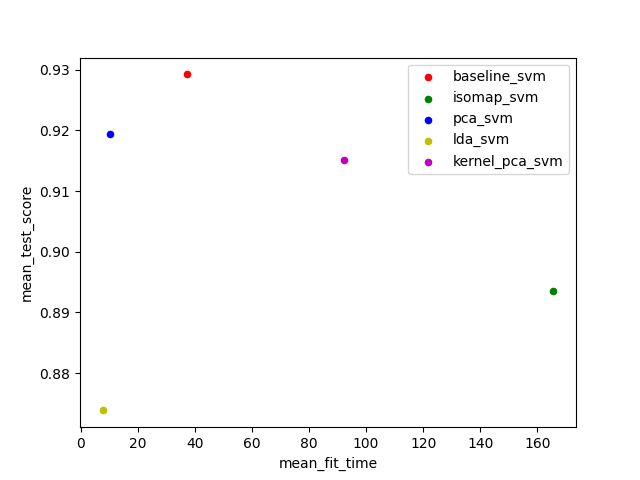
\includegraphics[width=0.8\textwidth]{figures/1-experiment/experiment1_plot.png}
    \caption{graph of time(in seconds) and accuracy(in percentage) for different dimensionality reduction methods}
    \label{fig:discussion-experiment-1-plot}
\end{figure}

When using \gls{lda} on 15000 samples, the accuracy falls to 88.76\%, but it only takes 7 seconds to train the model. \gls{lda} has a swift training time but low accuracy, but one thing to note, is that the maximum number of dimensions \gls{lda} can reduce to is 9 in this context. Therefore, the scores for \gls{lda} are worse than any dimensionality reduction method used. As the other methods use 49 dimensions to reduce the data, which is much higher than 9, it makes sense that the accuracy is higher than \gls{lda}. \gls{lda} only takes 7 seconds to train the model, so it is an excellent method to use if one wants a fast model with lower accuracy by comparing the other methods with more dimensions. 

When using 60000 samples, the accuracy is 89.33\%, and it takes 58 seconds to train the model. This means that the time it takes to train the model grows 728,57\% by using 45000 more examples of data. This is a big difference in time but a slight difference in accuracy; however, \gls{lda} is the fastest method, with lower accuracy than other methods. By using \gls{lda}, the model is faster but comes with the cost of lower accuracy.

When using \gls{pca} on 15000 samples, the accuracy is 92.37\%, and it takes 10 seconds to train the model, which is faster than the baseline \gls{svm} alone but still slower than \gls{lda} with the same amount of samples. When using 60000 samples, the accuracy is 93.25\%, and it takes 97 seconds to train the model. This means that the time it takes to train the model grows by 870\% by using 45000 more data samples. \gls{pca} has a lower accuracy than the baseline \gls{svm}. It is still faster than \gls{svm} alone but slower than \gls{lda}, making the model a good choice if one wants a faster model with slightly lower accuracy than the baseline \gls{svm}.

When using \gls{kpca} on 15000 samples, the accuracy is 92.36\%, and it takes 92 seconds to train the model. \gls{kpca} is slower than the baseline \gls{svm} and linear methods; this makes sense since nonlinear dimensionality methods can be heavier to compute. Nevertheless, \gls{kpca} scores the highest accuracy of all the dimensionality reduction methods used when using 15000 samples. If the computational cost is not an issue, \gls{kpca} is the best dimensionality reduction.

When using \gls{isomap} on 15000 samples, the accuracy is 90.61\%, and it takes 165 seconds to train the model. \gls{isomap} is slower than all the other dimensionality reduction methods and the baseline \gls{svm}. This makes sense since nonlinear dimensionality methods can be heavier to compute. However, \gls{isomap} scores the second lowest accuracy of all the dimensionality reduction methods used when using 15000 samples. So there are better dimensionality reduction methods than \gls{isomap} if one wants a fast model with high accuracy.

To conclude from this experiment, the baseline \gls{svm} is the best model to use if one wants a fast model with high accuracy. If one wants a faster model with lower accuracy, \gls{lda} is the best model to use. If one wants a model with high accuracy but slower than the baseline \gls{svm}, \gls{kpca} is the best model. If one wants a model with high accuracy but slower than the baseline \gls{svm}, \gls{isomap} is the best model. \gls{pca} is the best model if one wants a model with high accuracy and faster than the baseline SVM.

\subsubsection{F1-scores}\label{subsec:discussion-experiment-1-f1-score}
One thing to note is that the f1-score is the harmonic mean of precision and recall, which means that the f1-score is the average of the precision and recall. The f1-score is an excellent metric to use when the classes need to be balanced, as it is the average of precision and recall.
\begin{table}
    \centering
    \begin{tabular}{llrrr}
        \hline
        Reduction method & f1-score & worst score & 2. worst score & 3. worst score \\
        \hline
        \gls{svm}-15 & 93.43\% & 5 & 3 & 8 \\
        \gls{svm}-60 & 94.47\% & 5 & 8 & 3 \\
        \gls{lda}-15 & 88.59\% & 8 & 5 & 9 \\
        \gls{lda}-60 & 89.16\% & 8 & 5 & 3 \\
        \gls{pca}-15 & 92.25\% & 5 & 8 & 3 \\
        \gls{pca}-60 & 93.14\% & 5 & 3 & 8 \\
        \gls{kpca}-15 & 92.22\% & 5 & 3 & 9 \\
        \gls{isomap}-15 & 90.50\% & 9 & 8 & 7 \\
        \hline
    \end{tabular}
    \caption{F1-scores for the different dimensionality reduction methods.}
    \label{tab:discussion-experiment-1-f1-score}
    \end{table}
All experiments are displayed in Table \ref{tab:discussion-experiment-1-f1-score}, which shows the f1-score for the different models and the three worst classes for f1-scores.
In all experiments done, all of the models have a high f1-score, which means that the models are good at recognizing the numbers in the pictures. all models are best at recognizing zeros and ones in pictures. and good at recognizing four and sixes. When it comes to what the different models are bad at distinguishing, it is different for all. The most common number that the models are bad at recognizing is threes, fives, and eights, in a different order depending on the dimensionality reduction method used as these are the worst in \gls{svm} with both 15000 and 60000 samples, \gls{lda} with 60000 samples, \gls{pca} with 15000 samples and 60000 samples. \gls{isomap} is the only model that could be better at recognizing threes or fives, as it is terrible at sevens, eights, and nines. This can impact if one wants to use the model to find threes or fives; \gls{isomap} can be considered, as it is good at recognizing these numbers.

\gls{lda} with 15000 samples is interesting, as it needs to improve recognizing fives, eights, and nines. This is interesting as \gls{lda} with 60000 samples needs to improve recognizing threes, fives, and eights. This means \gls{lda} gets better at recognizing nines. This can be because more nines come into the dataset using 60000 samples, which makes \gls{lda} better at recognizing nines. 

In the occasions where there is more than one experiment done to the same method, the worst f1-scores for a class change, as seen in \gls{pca}, where at 15000 samples, the eights have the second worst f1-score, but at 60000 samples, the eights have the third worst f1-score. So the worst f1-scores for a class can change depending on the number of samples used.

To conclude this experiment, the models are good at recognizing the numbers in the pictures, but they are not perfect. The models are best at recognizing zeros and ones in pictures and recognizing four and sixes. When it comes to what the different models are bad at distinguishing, it is different for all. The most common number that the models are bad at recognizing is threes, fives, and eights, in a different order depending on the dimensionality reduction method used as these are the worst in \gls{svm} with both 15000 and 60000 samples, \gls{lda} with 60000 samples, \gls{pca} with 15000 samples and 60000 samples. \gls{isomap} is the only model that is not bad at recognizing threes or fives, as it is terrible at sevens, eights, and nines. This can have an impact if one wants to use the model to find threes or fives, \gls{isomap}P can be considered, as it is not bad at recognizing these numbers, but if one wants to use the model to find eights, then \gls{isomap} is not a good choice.

%intro
%presentation af de experimenter vi har valgt og hvorfor vi har valgt dem?
% experiment 1 exemple
%     detaljeret gennemgang af regler og evaluering
%     fremvisning af resultater
%     opsumering af resultater
%     diskussion af resultater og hvad der ellers var spændende evaluering af hvorfor det blev sådan.
%why this experiment was chosen
%look at f1-score and accuracy and time fitting the data
\section{Experiment 2}\label{sec:experiment-2}
This section will describe the second experiment of the project. The second experiment covers the necessary dimensions before reaching a threshold of 1\%, 5\%, and 10\% loss of accuracy. The experiment will only be done on 15.000 samples, instead of the entire dataset of 60.000 samples, due to issues regarding memory usage. The experiment will focus on when different dimensionality reduction methods drop in accuracy due to too few dimensions and compare them to each other to display the robustness of each of the methods.


\subsection{Rules and overview of the experiment}\label{subsec:experiment_2_rules}
This section will cover the rules of the second experiment and how the experiment results will be evaluated.

Every test in the second experiment is run on the same computer, pc-1. See \autoref{tab:pc1-specs} for the specific specs for the computer used in the experiment. It was first tried to run on another pc with less memory, but it was found that the nonlinear methods would take too long to run, and therefore it was run on pc-1.

For this experiment, the number of components will vary from around 2/5 to 50, and this range was chosen as it was believed to have a sufficient amount of components to show a general trend. For the nonlinear methods, 5 components, instead of 2, were chosen as the lowest amount, as the nonlinear methods gave errors when using fewer components than 5.

\gls{lda} is an exception, as the maximum number of components is the number of classes $-1$, which is 9 for the \gls{mnist} dataset, which means that the range of components for \gls{lda} will be from 2-9.

The values used to evaluate this experiment are \texttt{mean\_test\_score} based on \texttt{param\_pca\_\_n\_components} to evaluate the model's accuracy with the number of components used.

For each experiment, the data will be analyzed to see how many components can be removed before the accuracy drops below a certain threshold. For the experiment's sake, the thresholds will be based on the best accuracy score for each method. The thresholds will be a 1\% loss in accuracy, a 5\% loss in accuracy, and a 10\% loss in accuracy. If a method has the best accuracy score of 96\%, the thresholds will be 96 - 1\% = 95.05, 96 - 5\% = 91.20, and 96 - 10\% = 86.40. These thresholds were chosen as they are believed to be a good balance between the number of components that can be removed and the amount of accuracy lost, which could be acceptable for some use cases.


\subsection{Results}\label{subsec:experiment_2_results}
This section will cover the results gathered from running the second experiment. Each of the dimensionality reduction methods will be presented using scatter plots. The scatter plots will show the number of components used along the x-axis and the model's accuracy along the y-axis. Each component has multiple dots, so the accuracy varies slightly depending on the hyperparameters used, but the general trend is the same. The results will then be compared and evaluated based on the experiment's rules.

The main focus of the evaluation will be on when the accuracy starts to drop noticeably and how many components are needed to have good accuracy still. The scatter plots are used to represent the results visually, and the specific values of the accuracy will also be discussed. These values are taken from the csv files generated from running the second experiment.

\subsubsection{\gls{pca}}\label{subsubsec:experiment_2_pca}
\gls{pca} is a linear dimensionality reduction method; the scatter plot representing this method can be seen in \autoref{fig:experiment_2_pca_svm}.

As one would expect, the model's accuracy increases as the number of components increases. However, around 20 components, the accuracy starts to drop, the accuracy especially has a noticeable drop between 10 and 20 components, and the accuracy has a drastic drop for each component removed below ten components. This is expected as the lower the number of components the model has to work with; the more information is lost.

\begin{figure}[htb!]
    \centering
    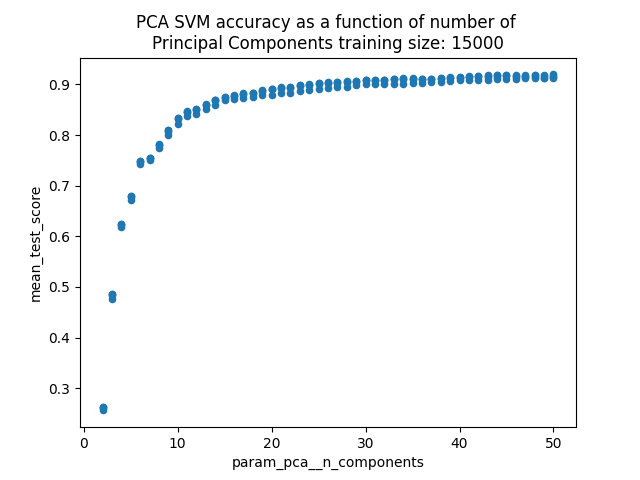
\includegraphics[width=0.8\textwidth]{figures/experiment_two/pca_svm_15000.png}
    \caption{Accuracy of the SVM model with \gls{pca} as dimensionality reduction method, with the number of components used.}
    \label{fig:experiment_2_pca_svm}
\end{figure}

For \gls{pca}, the highest accuracy value is 91.99\% with 50 components and the value 0.01 for the C hyperparameter in \gls{svm}. The thresholds for \gls{pca} are: 91.99 - 1\% = 91.07, 91.99 - 5\% = 87.39, and 91.99 - 10\% = 82.79. The results of the experiment for \gls{pca} will be compared to these thresholds.

By sorting the data by \texttt{mean\_test\_score} and going through the values, given the best-case scenario with the best hyperparameters found. The first value that drops below the threshold of 91.07\% is with an accuracy of 90.57\% at 29 components, which means that the model's accuracy only increases by 1\% with the last 21 components, which is close to half the total amount of components.
The next threshold of 87.39\% accuracy is found at 86.86\% with 14 components. By removing an additional seven components, the accuracy dropped from a 1\% loss to a 5\% loss.
The final threshold of 82.79\% accuracy is found at 80.70\% with nine components. By removing only five components, the accuracy dropped from a 5\% loss to a 10\% loss.

\subsubsection{Linear discriminant analysis}\label{subsubsec:experiment_2_lda}
The scatter plot representing \gls{lda} method can be seen in \autoref{fig:experiment_2_lda_svm}. \gls{lda} reduces the dimension to the number of classes $-1$, which is why the total number of components used is nine since \gls{mnist} has ten different numbers. The general trend is still valid for discussion in the second experiment.


\begin{figure}[htb!]
    \centering
    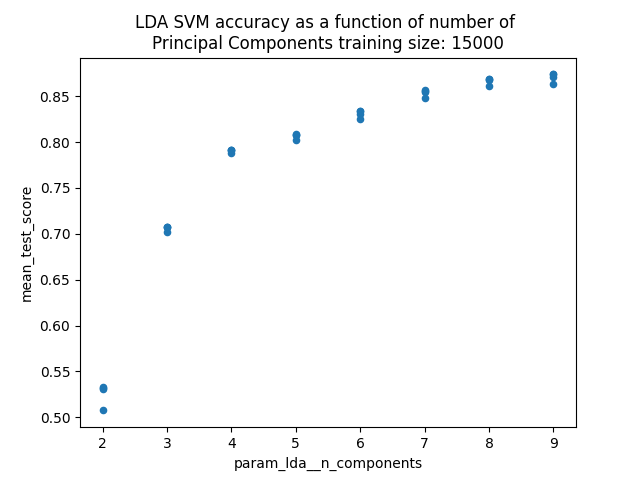
\includegraphics[width=0.8\textwidth]{figures/experiment_two/lda_svm_15000.png}
    \caption{Accuracy of the SVM model with \gls{lda} as dimensionality reduction method, with the number of components used.}
    \label{fig:experiment_2_lda_svm}
\end{figure}

For \gls{lda}, the highest accuracy score is at 87.38\% with nine components and the value 0.1 for the C hyperparameter in \gls{svm}. The thresholds for \gls{lda} are: 87.38 - 1\% = 86.50, 87.38 - 5\% = 83.01, and 87.38 - 10\% = 78.64. The experiment's results for \gls{lda} will be compared to these thresholds.

Repeating the method of looking through the data gathered, the first value that drops below the first threshold  of 86.50\%, with the 0.1 hyperparameter, is at 85.61\% with seven components.

The next threshold of 83.01\% accuracy is found at 80.83\% with five components. By removing two components, the accuracy dropped from a 1\% loss to a 5\% loss, which is not many components when compared to \gls{pca}, but for \gls{lda} that only has nine total components, a large percentage of the components can be removed with only a 5\% accuracy loss.

The final threshold of 78.64\% accuracy is found at 70.75\% with only three components. They are showing a significant drop from the threshold since the first few components impact the accuracy score significantly, and the closest value to the threshold is ~8\% away.


\subsubsection{\gls{kpca}}\label{subsubsec:experiment_2_kpca}
\gls{kpca} is a nonlinear dimensionality reduction method, and the scatter plot representing this method can be seen in \autoref{fig:experiment_2_kpca_svm}.

\begin{figure}[htb!]
    \centering
    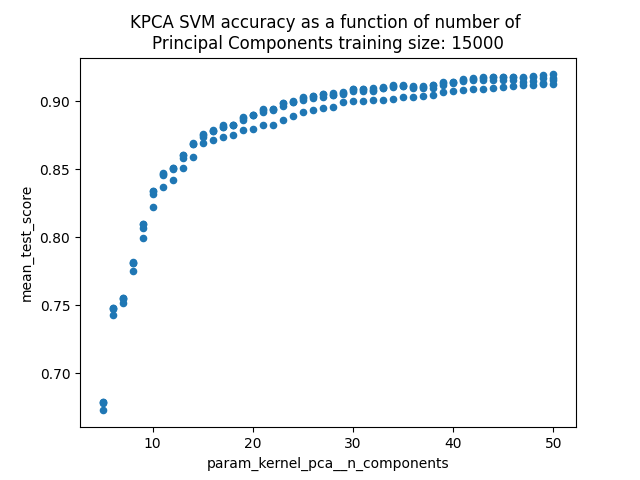
\includegraphics[width=0.8\textwidth]{figures/experiment_two/kpca_svm_15000.png}
    \caption{Accuracy of the SVM model with \gls{kpca} as dimensionality reduction method, with the number of components used.}
    \label{fig:experiment_2_kpca_svm}
\end{figure}

\autoref{fig:experiment_2_kpca_svm} is very similar to the other methods, and almost identical with \autoref{fig:experiment_2_pca_svm}, the only difference is that \gls{kpca} uses at minimum 5 components, where \gls{pca} uses at the lowest 2 components.

\gls{kpca} has a top accuracy score of 91.99\% with the value 0.01 for the C hyperparameter in \gls{svm}, meaning that the thresholds for \gls{kpca} are: 91.99 - 1\% = 91.07, 91.9 - 5\% = 87.39, and 91.9 - 10\% = 82.79. The experiment's results for \gls{kpca} will be compared to these thresholds.

Similar to linear methods, the data is sorted by its accuracy score to find the first value where the accuracy drops below a threshold, that uses the same hyperparameter. The first threshold of 91.07\% accuracy is found at 91.04\% with 34 components. The next threshold of 87.39\% accuracy is found at 86.86\% with 14 components. The final threshold of 82.79\% accuracy is found at 80.70\% with nine components.


\subsubsection{\gls{isomap}}\label{subsubsec:experiment_2_isomap}
\gls{isomap} is the final method of the second experiment, which is nonlinear, and the scatter plot representing this method can be seen in \autoref{fig:experiment_2_isomap_svm}.

\begin{figure}[htb!]
    \centering
    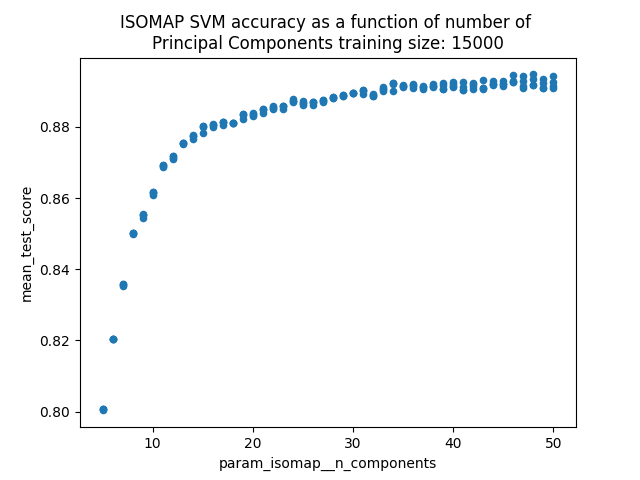
\includegraphics[width=0.8\textwidth]{figures/experiment_two/isomap_rerun_svm_15000.png}
    \caption{Accuracy of the SVM model with \gls{isomap} as dimensionality reduction method, with the number of components used.}
    \label{fig:experiment_2_isomap_svm}
\end{figure}

\autoref{fig:experiment_2_isomap_svm} is similar to the other methods as the accuracy drops drastically as the number of components decreases, but interestingly even the lowest accuracy for \gls{isomap} is still relatively high. The span from best to worst accuracy is much smaller than the other methods. The highest accuracy score for \gls{isomap} is 89.4\% with 48 components and the value 0.001 for the C hyperparameter in \gls{svm}, and the lowest accuracy score is 80\% with five components. The best and worst accuracy scores are closer together than the other methods, with only a ~9\% difference.

isomap has a top accuracy score of 89.47\%, with 48 components, and the value 0.001 for the C hyperparameter in \gls{svm}. meaning that the thresholds for \gls{isomap} are: 89.47 - 1\% = 88.57, 89.47 - 5\% = 84.99, and 89.47 - 10\% = 80.52.

The first threshold of 88.57\% accuracy is found at 88.49\% with 22 components, the next threshold of 84.99\% accuracy is found at 83.54\% with seven components, and the final threshold of 79.4\% accuracy is not found in the data, as the lowest accuracy score is 80.8\% with five components. To still be able to compare the results of \gls{isomap}  with the other methods, the lowest accuracy score will be used as the threshold, but it should be made clear that the actual threshold is not found in the data.


\subsection{Discussion of experiment 2}\label{subsec:experiment_2_discussion}
This section will discuss the results of the second experiment and compare the results of the different methods, first by discussing the results of the linear methods, then the nonlinear methods, and finally, comparing the results of all methods.

For each section, a table will display the different percentages of components remaining before the accuracy drops below a threshold. The table will also show the number of remaining components to show the difference between the methods.


\subsubsection{Linear methods}
By comparing the two linear methods used for the second experiment, it is essential to know that the number of components is very different between \gls{pca} \gls{lda}, which means that an exact comparison between the two methods is not always clear. Instead of using the number of components as a comparison, the percentage of remaining components will be used to try and make a fair comparison. A table showing the differences between the two methods can be seen in \autoref{tab:experiment_2_linear_methods_comparison}.

\begin{table}[htb!]
    \centering
    \begin{tabular}{cp{0.15\textwidth}p{0.15\textwidth}}
        \toprule
        \textbf{Thresholds} & \textbf{PCA \% 50} & \textbf{LDA \% 9} \\
        \midrule
        1\%                 & 58\% (29)          & 77.7\% (7)        \\
        5\%                 & 28\% (14)          & 55.5\% (5)        \\
        10\%                & 18\% (9)           & 33.3\% (3)        \\
        \bottomrule
    \end{tabular}
    \caption{Percentage of the components remaining after the threshold is reached, with the corresponding number of components in paratheses.}
    \label{tab:experiment_2_linear_methods_comparison}
\end{table}

\autoref{tab:experiment_2_linear_methods_comparison} shows, for each linear method, the amount of components left after each of the thresholds is reached. So for \gls{pca}, 58\% of the total number of components remain before reaching the first threshold of 1\%, whereas, for \gls{lda}, there is 77.7\%.

From \autoref{tab:experiment_2_linear_methods_comparison}, it can be seen that before reaching the first threshold of losing 1\% accuracy, \gls{pca} can cut off 42\% of its components, while \gls{lda} can can only cut off 22.3\%.

By comparing the two linear methods, it can be concluded that \gls{lda} is more prone to losing accuracy when removing components than \gls{pca}. The accuracy loss is likely because \gls{lda} has so few components to work with in the first place. It could be argued that the results are not entirely fair since \gls{pca} has so many more components, but scaling the values with percentage should show a general trend.


\subsubsection{nonlinear methods}
Unlike the linear methods, the nonlinear methods have a similar number of components, which should give a more fair comparison. A table showing when the respective thresholds were reached for each of the nonlinear methods can be seen in \autoref{tab:experiment_2_non_linear_methods_comparison}.

\begin{table}[htb!]
    \centering
    \begin{tabular}{cp{0.20\textwidth}p{0.20\textwidth}}
        \toprule
        \textbf{Thresholds} & \textbf{KPCA \% 50} & \textbf{ISOMAP \% 50} \\
        \midrule
        1\%                 & 68\% (34)           & 40\% (22)             \\
        5\%                 & 28\% (14)           & 14\% (7)              \\
        10\%                & 18\% (9)            & 1\% (5)*              \\
        \bottomrule
    \end{tabular}
    \caption{Percentage of the components remaining after the threshold is reached, with the corresponding number of components in paratheses.}
    \label{tab:experiment_2_non_linear_methods_comparison}
\end{table}

Figure 1 shows that \gls{kpca} and \gls{isomap} can afford to cut off a significant amount of components before reaching the first threshold of 1\%. \gls{kpca} can cut off 42\% of its components, while \gls{isomap} can cut off 60\% of its components. Another interesting note is that \gls{isomap} never reaches the 10\% accuracy loss threshold, and the closest accuracy score is used instead. Although it is not entirely accurate, the percentage from the actual threshold is <1\%, so for the sake of the comparison, it will be assumed that the threshold was reached.

Generally, it can be concluded that both \gls{kpca} and \gls{isomap} can afford to cut off a significant amount of components before losing accuracy. It is interesting to note that \gls{isomap} can cut off more components than \gls{kpca} before losing accuracy. However, \gls{kpca} reaches a higher accuracy score than \gls{isomap} but also reaches a lower accuracy score than \gls{isomap}, which means that \gls{isomap} could be considered more consistent than kpca, as the span of accuracy score for \gls{isomap} is smaller.


\subsubsection{Comparison of methods}
Now that the linear and nonlinear methods have been compared, it is time to compare the methods to each other. The results can be seen in \autoref{tab:experiment_2_methods_comparison}.


\begin{table}[htb!]
    \centering
    \begin{tabular}{cp{0.15\textwidth}p{0.15\textwidth}p{0.15\textwidth}p{0.20\textwidth}}
        \toprule
        \textbf{Thresholds} & \textbf{PCA \% 50} & \textbf{LDA \% 9} & \textbf{KPCA \% 50} & \textbf{ISOMAP \% 50} \\ \midrule
        1\%                 & 58\% (29)          & 77.7\% (7)        & 58\% (34)           & 40\% (22)             \\
        5\%                 & 28\% (14)          & 55.5\% (5)        & 28\% (14)           & 14\% (7)              \\
        10\%                & 18\% (9)           & 33.3\% (3)        & 18\% (9)            & 1\% (5)*              \\
        \bottomrule
    \end{tabular}
    \caption{Percentage of the components remaining after the threshold is reached, with the corresponding number of components in paratheses.}
    \label{tab:experiment_2_methods_comparison}
\end{table}

The first noticeable thing is that \gls{pca} and \gls{kpca} are similar in the number of components they can cut off before losing accuracy enough to reach the thresholds. The highest accuracy score is the same between the two methods, but the lowest accuracy score is lower for PCA, this lower accuracy score is likely due to the range of components \gls{pca} has.  The lower the percentage in \autoref{tab:experiment_2_methods_comparison}, the more components can be cut off without losing accuracy. So from this, it can be concluded that \gls{lda} is the method that has the most drastic accuracy loss when cutting off components. This is likely because \gls{lda} has so few components to work in the first place, and therefore it is more sensitive to the removal of components. \gls{isomap} is the method that has the most negligible accuracy loss when cutting off components. Additionally, \gls{isomap}'s worst accuracy score is better than any other method, but its best accuracy score is also the lowest.

From the second experiment, it can be concluded that \gls{isomap} is the method that can cut off most components before losing accuracy. However, each method has its strengths and weaknesses, and it is essential to consider the context of the problem when choosing a method.


% intro
% presentation af de experimenter vi har valgt og hvorfor vi har valgt dem?
% experiment 1 exemple
%     detaljeret gennemgang af regler og evaluering
%     fremvisning af resultater
%     opsumering af resultater
%     diskussion af resultater og hvad der ellers var spændende evaluering af hvorfor det blev sådan.

%logarithmic regression
%Bar chart
\section{Experiment 3}
This experiment is targetted towards \gls{pca} and \gls{kpca}. The goal is to compare the performance of \gls{pca} and \gls{kpca}, because these methods are similar, with the exception that \gls{kpca} implements a kernel. Beause of the similarity of the methods, comparison will be more focused on the impact the different kernels can have on the model, namely what numbers does the machine learning model confuse given the different kernels.


As explained in the Chapter Theory, KPCA can have kernels, which will project the data into a higher dimensional feature space, where a hyperplane can be constructed, and perform PCA on it. KPCA does not require the transformation of the inputs into the feature space with the kernel function, but can use the kernels so as to get the dot product of the pair-wise input points~\cite{kpca-book}.


The kernels are a measure of similarity between the points~\cite{scikit-learn}, which means that points that are close to each other have higher similarity score, which is computed with the kernel function. The kernels chosen for the experiment are the \gls{rbf} and sigmoid kernels. The sigmoid kernel \textcquote{scikit-learn}{computes the sigmoid kernel between two vectors}, which outputs a value between -1 and 1 for the two given input vectors. The \gls{rbf} kernel \textcquote{scikit-learn}{computes the radial basis function kernel between two vectors}, which outputs a value between 0 and 1.


\subsection{Rules}
This experiment will not use gridsearch. The input of the data samples will be 15000 for both of the methods, because of hardware limitations. The amount of components used for the methods will be the ones that were used in experiment one, namely 49 components. The evaluation will be based on the confusion matrices, and eventually also for the score of the methods. The kernels used will be \gls{rbf} and sigmoid.


\subsection{Results}
Figure \ref{fig:confusion-matrix-pca-svm} shows the results for \gls{pca}.
Figure~\ref{fig:confusion-matrix-kernel-pca-svm-sigmoid} shows the results for \gls{kpca} with sigmoid kernel.
Figure~\ref{fig:confusion-matrix-kernel-pca-svm-rbf} shows the results for \gls{kpca} with rbf kernel.


\begin{figure}[htb!]
    \centering
    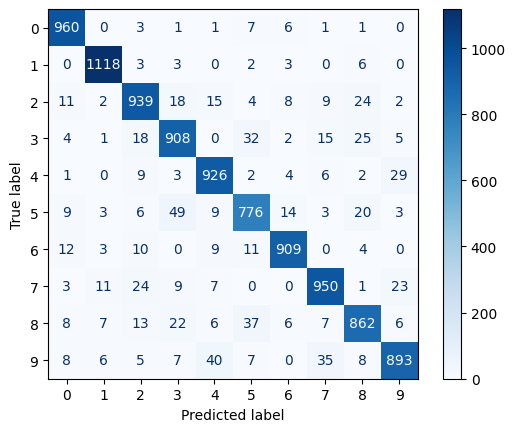
\includegraphics[width=0.5\textwidth]{../src/results/experiment_three/confusion_matrix_pca_svm.png}
    \caption{Confusion matrix for PCA}
    \label{fig:confusion-matrix-pca-svm}
\end{figure}





\begin{figure}
    \centering
    \subfloat[\centering Confusion matrix for kPCA Sigmoid]{\label{fig:confusion-matrix-kernel-pca-svm-sigmoid}{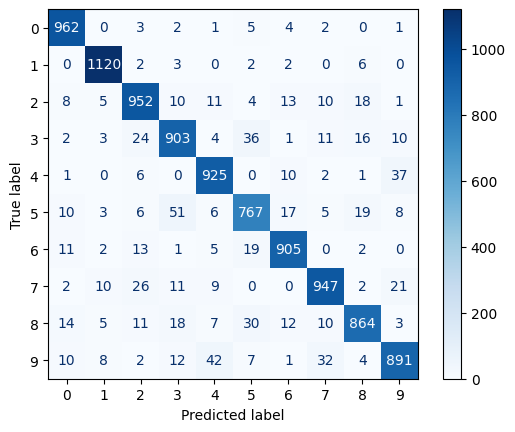
\includegraphics[width=0.45\textwidth]{../src/results/experiment_three/confusion_matrix_kernel_pca_svm_sigmoid.png} }}
    \qquad
    \subfloat[\centering Confusion matrix for kPCA RBF]{\label{fig:confusion-matrix-kernel-pca-svm-rbf}{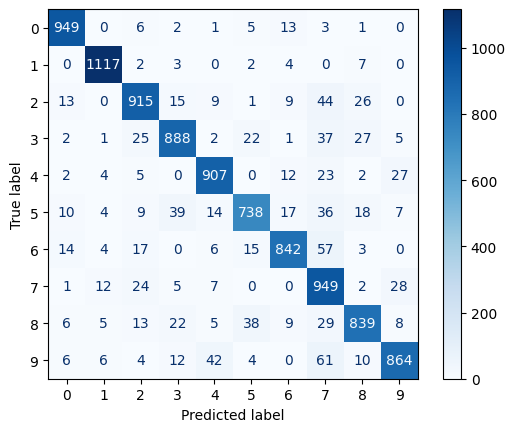
\includegraphics[width=0.45\textwidth]{../src/results/experiment_three/kernel_pca_rbf_kernel_49.png} }}%
    \caption{both kPCA kernels confusion matrices}
    \label{fig:kpca-kernels}
\end{figure}






\subsection{Results}
A slight improvement over the number 0 has been seen in \gls{kpca-s} in that it mapped 11 numbers better than \gls{pca}, and the same can be said for the number 2.

Both methods acquired the same amount of correct predictions for the numbers 3 and 4.

A slight difference appears in the number 5, where \gls{pca} has 780 correct predictions, and \gls{kpca-s} got 767, which is worse than \gls{pca}. The reason for that is because it confused it with the numbers 3 and 6.


A slight improvement in \gls{kpca-s} is seen at the number 6, where it got five numbers more than \gls{pca}. Such a low number is not worth considering, however.

It can be seen that sigmoid confuses the number 7 with the number 9 more often than \gls{pca} normally would, which worsens \gls{kpca-s}' ability to predict the number 7 correctly.

The notable impressions regarding the differences between \gls{pca} and \gls{kpca-s} are: \gls{kpca-s} improved by about ten numbers at the numbers 0 and 2, became worse at the number 5, became worse at the number 7, and shined the most at the number 8. The most interesting cases are the numbers 0,2, 5, and 8.


The RBF kernel has confused more number 2's than any other method presented in this experiment. As opposed to \gls{pca} and \gls{kpca-s}, \gls{kpca-r} confused it 33 times more with the number 7 and around ten times more with the number 8. The same pattern can be seen at the number 3, where it was again confused with numbers 7 and 8.


\gls{kpca-r} has confused the number 4 mainly with the numbers 7 and 9, and \gls{kpca-s} has only confused it with the number 9. Concerning the number 4, \gls{kpca-s} is the only method that has confused it the most with the number 9.


\gls{kpca-r} mainly confuses the number 5 with the numbers 3 and 7, whereas \gls{kpca-s} does it with the numbers 3, 6, and 8, and the same can be said about \gls{pca}.

The number 6 reveals a potentially interesting finding: \gls{kpca-r} is the only method that managed to confuse the number 6 with the number 7, as opposed to the other methods, which did not confuse it with the number 7.

The only place where \gls{kpca-r} outshines \gls{kpca-s} is at the number 7, where \gls{kpca-r} confuses with two numbers less than \gls{kpca-s}. Such a finding, however, is not of major importance because \gls{kpca-r} underperforms most of the time. 

\subsubsection{Summary of the differences between the methods}
From the results presented so far about the differences between the kernels it can be seen that all the methods often confuse the number 2 with 8; 3 with 2,5,8 and to a certain degree(PCA and much worse with \gls{kpca-r}), 7. The methods also confuse the number 4 with 9; 5 with 3,6, and 8 (\gls{kpca-r} also does it with 7). The number 6 gets confused with the number 0,2,5 (\gls{kpca-r} also does it with 7).
The number 7 gets confused with the number 2,3 and 9. \gls{kpca-r} is the only one that did not confuse the number 3 as much as the other methods.

At number 8, the methods have confused 0 (except for \gls{kpca-r}),2,3 and 5. \gls{kpca-r} confused it again with the number 7, but it is the only one that managed to map the number 0 less than the other methods. Lastly the number 9 got confused with the numbers the most with the numbers 4 and 7. It can be further noted that \gls{kpca-r} is the worst at confusing various numbers with the number 7.


From the overview provided regarding the difference in numbers, a percentage would be more preferable, more specifically, a percentage of the errors made in the numbers 0-9. Table \ref{tab:error-percentage-pca-kpca-s-kpca-r} shows the difference in percentages of errors made by the methods for each number.

\begin{table}[htb!]
    \centering
    \begin{tabular}{lrrrr}
        \toprule
          & pca    & kpca-s & kpca-r \\
        \midrule
        0 & 2.959  & 1.836  & 3.163  \\
        1 & 1.585  & 1.321  & 1.585  \\
        2 & 8.817  & 7.751  & 11.337 \\
        3 & 10.594 & 10.594 & 12.079 \\
        4 & 5.702  & 5.804  & 7.637  \\
        5 & 12.556 & 14.013 & 17.264 \\
        6 & 6.054  & 5.532  & 12.108 \\
        7 & 7.101  & 7.879  & 7.684  \\
        8 & 13.552 & 11.293 & 13.860 \\
        9 & 11.992 & 11.694 & 14.370 \\
        \bottomrule
    \end{tabular}
    \caption{Error percentage for each number for the methods}
    \label{tab:error-percentage-pca-kpca-s-kpca-r}
\end{table}

Another finding which could be explored is the difference in the number of errors made by the methods for each number. Table \ref{tab:error-percentage-pca-kpca-s-kpca-r} shows the difference in the number of errors made by the methods for each number.

Yet another finding that could be explored is to research why \gls{kpca-r} is the only method that confuses many numbers with the number 7.
%\subsection{Discussion of results}


\section{Experiment 4}\label{sec:experiment-4}

In this experiment, a machine learning pipeline is used to explore the effects of different sizes of samples on the performance of linear and non-linear dimensionality reduction methods. The \gls{mnist} data set is used as the source of data, and a range of sample sizes are selected, starting with 200 and ending with 5000. The pipeline uses \gls{svm} as the model and applies four different dimensionality reduction techniques: \gls{pca}, \gls{lda}, \gls{kpca}, and \gls{isomap}.

The performance of the pipeline is evaluated using three metrics: accuracy, f1-score, and time. The results of the experiment are analyzed to compare the performance of the different dimensionality reduction methods under varying sample sizes and to explore the differences between linear and non-linear approaches.

Overall, the results of this experiment provide insight into the factors that can influence the effectiveness of dimensionality reduction in machine learning and can inform the choice of dimensionality reduction method in real-world scenarios. Furthermore, the findings can contribute to the broader understanding of the role of sample size in the performance of machine learning models and dimensionality reduction.

\subsection{Parameters and evaluation}
In this experiment the same general hyper parameter tuning as in experiment 1 will be used on datasamples from \gls{mnist} of the size 200, 300, 400, 500, 600, 700, 800, 900, 1000, 2000, 3000, 4000, 5000. It will be evaluated based on f1, accuracy and how much time it uses.




\subsection{Results}\label{subsec:experiment_4_results}
In this section, we present the results of the fourth experiment, which compare the performance of different dimensionality reduction methods on a classification task. We show the results for different sample sizes using confusion matrices and tables, as well as scatter plots to visualize the relationship between sample size, accuracy, and time taken. We evaluate the results based on the rules of the experiment, focusing on accuracy, F1 score, time taken, and the size of the sample required to achieve good accuracy. We also discuss the specific values of accuracy obtained from the csv files generated by the experiment. The scatter plots provide a visual representation of the results and make it easy to see when accuracy and time start to improve. generally each method and the base case will show the results of the samples 200, 1000, 5000.

\subsubsection{\gls{svm} Model}\label{subsubsec:experiment_4_no_dimmensionality_reduction}

\begin{table}[htb!]
\centering
\begin{tabular}{lrrrr}
    \toprule
 & precision & recall & f1-score & support \\
 \midrule
 0 & 83.0224 & 90.8163 & 86.7446 & 980 \\
 1 & 78.2424 & 97.2687 & 86.7243 & 1135 \\
 2 & 67.8335 & 69.4767 & 68.6453 & 1032 \\
 3 & 73.6059 & 78.4158 & 75.9348 & 1010 \\
 4 & 70.7377 & 87.8819 & 78.3833 & 982 \\
 5 & 71.6243 & 41.0314 & 52.1739 & 892 \\
 6 & 91.3043 & 63.5699 & 74.9538 & 958 \\
 7 & 78.3178 & 81.5175 & 79.8856 & 1028 \\
 8 & 73.1092 & 71.4579 & 72.2741 & 974 \\
 9 & 71.7842 & 68.5828 & 70.1470 & 1009 \\
 accuracy & & & 756700 & 10000 \\
 macro avg & 75.9582 & 75.0019 & 74.5867 & 10000 \\
 weighted avg & 75.9485 & 75.6700 & 74.9591 & 10000 \\
 \bottomrule
\end{tabular}
\caption{Classification report for baseline\_svm\_200}
\label{tab:classification-report-baseline_svm_200}
\end{table}

\begin{table}[htb!]
\centering
\caption{Classification report for baseline_svm_1000}
\label{tab:classification-report-baseline_svm_1000}
\begin{tabular}{lrrrr}
\toprule
 & precision & recall & f1-score & support \\
\midrule
0 & 0.925998 & 0.970408 & 0.947683 & 980.000000 \\
1 & 0.921667 & 0.974449 & 0.947323 & 1135.000000 \\
2 & 0.865842 & 0.881783 & 0.873740 & 1032.000000 \\
3 & 0.877095 & 0.777228 & 0.824147 & 1010.000000 \\
4 & 0.867005 & 0.869654 & 0.868327 & 982.000000 \\
5 & 0.785340 & 0.840807 & 0.812128 & 892.000000 \\
6 & 0.914621 & 0.894572 & 0.904485 & 958.000000 \\
7 & 0.860927 & 0.885214 & 0.872902 & 1028.000000 \\
8 & 0.864350 & 0.791581 & 0.826367 & 974.000000 \\
9 & 0.822178 & 0.815659 & 0.818905 & 1009.000000 \\
accuracy & 0.871700 & 0.871700 & 0.871700 & 0.871700 \\
macro avg & 0.870502 & 0.870136 & 0.869601 & 10000.000000 \\
weighted avg & 0.871760 & 0.871700 & 0.871014 & 10000.000000 \\
\bottomrule
\end{tabular}
\end{table}

\begin{table}[htb!]
\centering
\begin{tabular}{lrrrr}
    \toprule
    & precision & recall & f1-score & support \\
    \midrule
    0 & 0.955224 & 0.979592 & 0.967254 & 980.000000 \\
    1 & 0.953072 & 0.984141 & 0.968357 & 1135.000000 \\
    2 & 0.909980 & 0.901163 & 0.905550 & 1032.000000 \\
    3 & 0.890279 & 0.915842 & 0.902879 & 1010.000000 \\
    4 & 0.904854 & 0.949084 & 0.926441 & 982.000000 \\
5 & 0.901278 & 0.869955 & 0.885339 & 892.000000 \\
6 & 0.952128 & 0.934238 & 0.943098 & 958.000000 \\
7 & 0.925123 & 0.913424 & 0.919236 & 1028.000000 \\
8 & 0.904555 & 0.856263 & 0.879747 & 974.000000 \\
9 & 0.902414 & 0.888999 & 0.895657 & 1009.000000 \\
accuracy & 0.920500 & 0.920500 & 0.920500 & 0.920500 \\
macro avg & 0.919891 & 0.919270 & 0.919356 & 10000.000000 \\
weighted avg & 0.920338 & 0.920500 & 0.920197 & 10000.000000 \\
\bottomrule
\end{tabular}
\caption{Classification report for baseline\_svm\_5000}
\label{tab:classification-report-baseline_svm_5000}
\end{table}


The first part of the experiment involved running a machine learning pipeline without applying any dimensionality reduction. The pipeline used a \gls{svm} model and was trained on the \gls{mnist} data set. The sample size for this part of the experiment was 100.

The results of this experiment are shown in \ref{tab:classification-report-baseline_svm_200}. The table shows the precision, recall, and f1-score for each of the ten classes in the data set, as well as the overall accuracy of the model. The table also shows the macro average and weighted average scores.

Overall, the results show that the \gls{svm} model achieved an accuracy of approximately 67\%. This indicates that the model performed relatively well but still had some errors in its predictions. The precision and recall scores for each class varied, with some classes having higher scores than others. For example, the model had a precision of approximately 87\% for class 0 but only a precision of approximately 45\% for class 9. 

These results provide a baseline for comparison with the results of the other parts of the experiment, in which different dimensionality reduction methods were applied. The results of this initial experiment will be used to evaluate the effectiveness of the different dimensionality reduction methods in improving the performance of the \gls{svm} model.

The second part of the base case involved using a sample size of 1000; it can be seen in \ref{tab:classification-report-baseline_svm_1000}. Compared to the results of the first part of the experiment, the accuracy of the \gls{svm} model improved significantly, achieving an accuracy of approximately 87\%. This indicates that using a larger sample size improved the performance of the model. The precision and recall scores for each class also improved, with most classes having higher scores than in the first part of the experiment.

The next sample of size 5000 can be seen in \ref{tab:classification-report-baseline_svm_5000}.
Comparing \ref{tab:classification-report-baseline_svm_5000} and \ref{tab:classification-report-baseline_svm_5000}, it is clear that the \gls{svm} model achieved higher accuracy and precision when trained on a larger sample size. For example, the accuracy of the model increased from 87\% for the 1000-sample data set to 92\% for the 5000-sample data set. Similarly, the precision of the model increased for most of the classes, with the largest increase being seen for class 5, where the precision increased from 78\% to 90\%.

Additionally, the f1-score, which is a measure of the balance between precision and recall, also improved for most classes when using a larger sample size. This suggests that the model was able to make more accurate predictions and avoid false positives and false negatives more effectively when trained on a larger data set.


\subsubsection{\gls{pca}}\label{subsubsec:experiment_4_pca}

The second part of the experiment involved running a machine learning pipeline applying \gls{pca} as a dimensionality reduction method. The sample sizes for this part of the experiment were 200, 1000, and 5000.

\begin{table}[htb!]
    \centering
    \begin{tabular}{lrrrr}
        \toprule
        & precision & recall & f1-score & support \\
        \midrule
        0 & 0.838207 & 0.877551 & 0.857428 & 980.000000 \\
        1 & 0.770701 & 0.959471 & 0.854788 & 1135.000000 \\
        2 & 0.675052 & 0.624031 & 0.648540 & 1032.000000 \\
        3 & 0.744227 & 0.829703 & 0.784644 & 1010.000000 \\
        4 & 0.692244 & 0.845214 & 0.761119 & 982.000000 \\
        5 & 0.747492 & 0.501121 & 0.600000 & 892.000000 \\
        6 & 0.931649 & 0.654489 & 0.768853 & 958.000000 \\
        7 & 0.832487 & 0.797665 & 0.814704 & 1028.000000 \\
        8 & 0.737317 & 0.671458 & 0.702848 & 974.000000 \\
        9 & 0.641791 & 0.724480 & 0.680633 & 1009.000000 \\
        accuracy & 0.754000 & 0.754000 & 0.754000 & 0.754000 \\
        macro avg & 0.761117 & 0.748518 & 0.747356 & 10000.000000 \\
        weighted avg & 0.760509 & 0.754000 & 0.750028 & 10000.000000 \\
        \bottomrule
    \end{tabular}
    \caption{Classification report for pca\_svm\_200}
    \label{tab:classification-report-pca_svm_200}
\end{table}


This classification report shows the performance of a \gls{svm} model that has been trained using \gls{pca}. The result of the first sample of 200 can be seen in \ref{tab:classification-report-pca_svm_200}
For example, class 0 has a precision of 0.838207 and a recall of 0.877551, while class 9 has a precision of 0.641791 and a recall of 0.724480. This indicates that the model is more accurate at correctly identifying instances of class 0 than it is at correctly identifying instances of class 9. The f1-score for class 0 is 0.857428, while the f1-score for class 9 is 0.680633, further highlighting the difference in performance between the two classes. Overall, it appears that class 0 and class 9 have the largest differences in performance on this classification report.


\begin{table}[htb!]
    \centering
    \begin{tabular}{lrrrr}
        \toprule
        & precision & recall & f1-score & support \\
        \midrule
        0 & 0.917235 & 0.961224 & 0.938714 & 980.000000 \\
        1 & 0.926271 & 0.962996 & 0.944276 & 1135.000000 \\
        2 & 0.880611 & 0.893411 & 0.886965 & 1032.000000 \\
    3 & 0.876923 & 0.790099 & 0.831250 & 1010.000000 \\
    4 & 0.900826 & 0.887984 & 0.894359 & 982.000000 \\
    5 & 0.789038 & 0.855381 & 0.820871 & 892.000000 \\
    6 & 0.915565 & 0.939457 & 0.927357 & 958.000000 \\
    7 & 0.902119 & 0.869650 & 0.885587 & 1028.000000 \\
    8 & 0.845890 & 0.760780 & 0.801081 & 974.000000 \\
    9 & 0.815414 & 0.849356 & 0.832039 & 1009.000000 \\
    accuracy & 0.878200 & 0.878200 & 0.878200 & 0.878200 \\
    macro avg & 0.876989 & 0.877034 & 0.876250 & 10000.000000 \\
    weighted avg & 0.878426 & 0.878200 & 0.877565 & 10000.000000 \\
    \bottomrule
\end{tabular}
\caption{Classification report for pca\_svm\_1000}
\label{tab:classification-report-pca_svm_1000}
    \end{table}

In \ref{tab:classification-report-pca_svm_1000} we can see that overall, the second model (pca\_svm\_1000) performs better on the classification task than the first model (pca\_svm\_200), as shown by the higher accuracy, precision, recall, and f1-score values for most classes in the second report. For example, class 0 has a precision of 0.917235 and a recall of 0.961224 in the second report, compared to 0.838207 and 0.877551 in the first report. The f1-score for class 0 is also higher in the second report (0.938714) than in the first report (0.857428).

One interesting difference between the two reports is the performance on class 3. In the first report, class 3 has a recall of 0.829703, with an f1-score of 0.784644. In the second report, class 3 a lower recall of 0.790099, resulting in a f1-score of 0.831250. This indicates that the second model (pca\_svm\_1000) is less accurate at correctly identifying instances of class 3 than the first model the f1 score is still higher due to the precision being suitably higher to compensate(pca\_svm\_200).

The last model is seen in \ref{tab:classification-report-pca_svm_5000} and is overall, the pca\_svm\_5000 model appears to have better performance across most of the metrics, with higher values for precision, recall, and f1-score for most of the classes. This indicates that the pca\_svm\_5000 model is more accurate at predicting the correct class for a given input.

\begin{table}[htb!]
    \centering
    \begin{tabular}{lrrrr}
        \toprule
    & precision & recall & f1-score & support \\
    \midrule
    0 & 0.940476 & 0.967347 & 0.953722 & 980.000000 \\
    1 & 0.958656 & 0.980617 & 0.969512 & 1135.000000 \\
    2 & 0.890927 & 0.894380 & 0.892650 & 1032.000000 \\
    3 & 0.866218 & 0.891089 & 0.878477 & 1010.000000 \\
    4 & 0.907389 & 0.937882 & 0.922384 & 982.000000 \\
    5 & 0.876417 & 0.866592 & 0.871477 & 892.000000 \\
    6 & 0.936259 & 0.935282 & 0.935770 & 958.000000 \\
    7 & 0.925000 & 0.899805 & 0.912229 & 1028.000000 \\
    8 & 0.897577 & 0.836756 & 0.866100 & 974.000000 \\
    9 & 0.891348 & 0.878097 & 0.884673 & 1009.000000 \\
    accuracy & 0.910000 & 0.910000 & 0.910000 & 0.910000 \\
    macro avg & 0.909027 & 0.908785 & 0.908699 & 10000.000000 \\
    weighted avg & 0.909832 & 0.910000 & 0.909711 & 10000.000000 \\
    \bottomrule
\end{tabular}
\caption{Classification report for pca-svm-5000}
\label{tab:classification-report-pca_svm_5000}
    \end{table}


Overall, the results show that the \gls{svm} model using \gls{pca} achieved an accuracy of approximately 75\%, 77\%, and 84\% for the 200, 1000, and 5000 sample sizes, respectively. This indicates that the model performed relatively well, but still had some errors in its predictions. The precision and recall scores for each class varied, with some classes having higher scores than others. For example, the model had a precision of approximately 83\% for class 0 with a 200 sample size, but only a precision of approximately 64\% for class 9 with a 1000 sample size.

The results show that the model performed better with larger sample sizes, as evidenced by the higher overall accuracy and f1-scores. In particular, classes 0 and 9 showed the largest differences in performance across the different sample sizes. Overall, the experiment demonstrates the importance of using a sufficient amount of data for training machine learning models.

\subsubsection{\gls{lda}}\label{subsubsec:experiment_4_lda}

\begin{table}[htb!]
    \centering
    \begin{tabular}{lrrrr}
        \toprule
    & precision & recall & f1-score & support \\
    \midrule
    0 & 0.801397 & 0.819388 & 0.810293 & 980.000000 \\
    1 & 0.604938 & 0.949780 & 0.739116 & 1135.000000 \\
    2 & 0.514586 & 0.427326 & 0.466914 & 1032.000000 \\
    3 & 0.667053 & 0.569307 & 0.614316 & 1010.000000 \\
    4 & 0.606034 & 0.695519 & 0.647700 & 982.000000 \\
    5 & 0.481481 & 0.204036 & 0.286614 & 892.000000 \\
    6 & 0.722449 & 0.554280 & 0.627289 & 958.000000 \\
    7 & 0.749458 & 0.672179 & 0.708718 & 1028.000000 \\
    8 & 0.590597 & 0.619097 & 0.604511 & 974.000000 \\
    9 & 0.437595 & 0.569871 & 0.495050 & 1009.000000 \\
    accuracy & 0.616200 & 0.616200 & 0.616200 & 0.616200 \\
    macro avg & 0.617559 & 0.608078 & 0.600052 & 10000.000000 \\
    weighted avg & 0.618068 & 0.616200 & 0.604480 & 10000.000000 \\
    \bottomrule
\end{tabular}
\caption{Classification report for lda\_svm\_200}
\label{tab:classification-report-lda_svm_200}
    \end{table}

This classification report seen in \ref{tab:classification-report-lda_svm_200} shows the performance of a \gls{svm} model that has been trained using \gls{lda} on classifying handwritten digits from the \gls{mnist} data set. For example, class 1 has a precision of 0.604938 and a recall of 0.949780, while class 5 has a precision of 0.481481 and a recall of 0.204036. This indicates that the model is more accurate at correctly identifying instances of class 1 than it is at correctly identifying instances of class 5. The f1-score for class 1 is 0.739116, while the f1-score for class 5 is 0.286614, further highlighting the difference in performance between the two classes. Overall, it appears that class 1 and class 5 have the largest differences in performance on this classification report.

\begin{table}[htb!]
    \centering
    \begin{tabular}{lrrrr}
        \toprule
        & precision & recall & f1-score & support \\
        \midrule
        0 & 0.699825 & 0.818367 & 0.754468 & 980.000000 \\
        1 & 0.745657 & 0.945374 & 0.833722 & 1135.000000 \\
        2 & 0.677530 & 0.382752 & 0.489164 & 1032.000000 \\
        3 & 0.625000 & 0.519802 & 0.567568 & 1010.000000 \\
        4 & 0.629767 & 0.689409 & 0.658240 & 982.000000 \\
        5 & 0.496101 & 0.570628 & 0.530761 & 892.000000 \\
        6 & 0.662461 & 0.657620 & 0.660031 & 958.000000 \\
        7 & 0.648130 & 0.657588 & 0.652825 & 1028.000000 \\
        8 & 0.594987 & 0.463039 & 0.520785 & 974.000000 \\
        9 & 0.552239 & 0.623389 & 0.585661 & 1009.000000 \\
        accuracy & 0.636700 & 0.636700 & 0.636700 & 0.636700 \\
        macro avg & 0.633170 & 0.632797 & 0.625323 & 10000.000000 \\
        weighted avg & 0.636121 & 0.636700 & 0.628514 & 10000.000000 \\
        \bottomrule
    \end{tabular}
    \caption{Classification report for lda-svm-1000}
    \label{tab:classification-report-lda_svm_1000}
\end{table}

The classification report for lda\_svm\_1000 seen in \ref{tab:classification-report-lda_svm_1000} shows generally better performance than the classification report for lda\_svm\_200. For example, class 1 has a precision of 0.745657 and a recall of 0.945374 in the lda\_svm\_1000 report, compared to a precision of 0.604938 and a recall of 0.949780 in the lda\_svm\_200 report. Additionally, the f1-score for class 1 is 0.833722 in the lda\_svm\_1000 report, compared to 0.739116 in the lda\_svm\_200 report. This indicates that the model trained on a larger sample size of 1000 has improved performance in correctly identifying instances of class 1. Overall, it appears that several classes, including 1, 3, 5, and 9, have seen improvements in precision, recall, and f1-score when trained on a larger sample size.


\begin{table}[htb!]
    \centering
    \begin{tabular}{lrrrr}
        \toprule
     & precision & recall & f1-score & support \\
    \midrule
    0 & 0.920039 & 0.951020 & 0.935273 & 980.000000 \\
    1 & 0.907577 & 0.960352 & 0.933219 & 1135.000000 \\
    2 & 0.871277 & 0.793605 & 0.830629 & 1032.000000 \\
    3 & 0.854692 & 0.838614 & 0.846577 & 1010.000000 \\
    4 & 0.827977 & 0.892057 & 0.858824 & 982.000000 \\
    5 & 0.806306 & 0.802691 & 0.804494 & 892.000000 \\
    6 & 0.881178 & 0.874739 & 0.877947 & 958.000000 \\
    7 & 0.869347 & 0.841440 & 0.855166 & 1028.000000 \\
    8 & 0.806999 & 0.781314 & 0.793949 & 974.000000 \\
    9 & 0.807843 & 0.816650 & 0.812223 & 1009.000000 \\
    accuracy & 0.856800 & 0.856800 & 0.856800 & 0.856800 \\
    macro avg & 0.855324 & 0.855248 & 0.854830 & 10000.000000 \\
    weighted avg & 0.856542 & 0.856800 & 0.856202 & 10000.000000 \\
    \bottomrule
\end{tabular}
\caption{Classification report for lda-svm-5000}
\label{tab:classification-report-lda_svm_5000}
\end{table}


The classification report for lda\_svm\_5000 has higher precision, recall, and f1-score values for each class compared to the lda\_svm\_1000 report. For example, the precision for class 0 is 0.920039 in the lda\_svm\_5000 report, while it is 0.699825 in the lda\_svm\_1000 report. Similarly, the recall for class 0 is 0.951020 in the lda\_svm\_5000 report, while it is 0.818367 in the lda\_svm\_1000 report. The f1-score for class 0 is also higher in the lda\_svm\_5000 report (0.935273) compared to the lda\_svm\_1000 report (0.754468). Overall, it appears that the model trained on a larger sample size is more effective at correctly classifying instances in the \gls{mnist} data set.

Based on these classification report, the model with \gls{lda} is best at recognizing instances of class 1. This is because it has the highest precision and recall among all classes, as well as the highest f1-score. This indicates that the model is able to accurately identify instances of class 1 with a high degree of precision and recall. Furthermore, the difference in performance between class 1 and other classes is the largest, further highlighting the model's superior performance on this class. It also appears that the model is worst at recognizing classes 8, 9, 2 and 5.

\subsubsection{\gls{kpca}}\label{subsubsec:experiment_4_kernel_pca}
In this part of the experiment we expect The performance of a \gls{svm} model using  \gls{kpca} for dimensionality reduction is likely to differ from that of an \gls{svm} model without \gls{kpca}. \gls{kpca} can reduce the dimensionality of a data set by projecting it onto a lower-dimensional space, which can improve the \gls{svm} model's decision boundary and performance. In contrast, an \gls{svm} model without \gls{kpca} may be more sensitive to the curse of dimensionality and overfitting, especially on high-dimensional data sets. 

\begin{table}[htb!]
    \centering
    \begin{tabular}{lrrrr}
        \toprule
        & precision & recall & f1-score & support \\
        \midrule
        0 & 0.752715 & 0.919388 & 0.827745 & 980.000000 \\
        1 & 0.687965 & 0.977093 & 0.807426 & 1135.000000 \\
        2 & 0.678387 & 0.635659 & 0.656328 & 1032.000000 \\
    3 & 0.707317 & 0.746535 & 0.726397 & 1010.000000 \\
    4 & 0.690129 & 0.818737 & 0.748952 & 982.000000 \\
    5 & 0.769231 & 0.426009 & 0.548341 & 892.000000 \\
    6 & 0.879245 & 0.729645 & 0.797490 & 958.000000 \\
    7 & 0.875664 & 0.801556 & 0.836973 & 1028.000000 \\
    8 & 0.793492 & 0.650924 & 0.715172 & 974.000000 \\
    9 & 0.705394 & 0.673935 & 0.689306 & 1009.000000 \\
    accuracy & 0.744100 & 0.744100 & 0.744100 & 0.744100 \\
    macro avg & 0.753954 & 0.737948 & 0.735413 & 10000.000000 \\
    weighted avg & 0.752395 & 0.744100 & 0.737969 & 10000.000000 \\
    \bottomrule
\end{tabular}
\caption{Classification report for kernel\_pca\_svm\_200}
\label{tab:classification-report-kernel_pca_svm_200}
\end{table}


The values in \ref{tab:classification-report-kernel_pca_svm_200} indicate that the model has relatively high precision and recall for most classes, with a few exceptions. Overall, the model has an accuracy of approximately 74\%.

\begin{table}[htb!]
    \centering
    \begin{tabular}{lrrrr}
        \toprule
        & precision & recall & f1-score & support \\
        \midrule
        0 & 0.912745 & 0.950000 & 0.931000 & 980.000000 \\
        1 & 0.926236 & 0.973568 & 0.949313 & 1135.000000 \\
        2 & 0.873466 & 0.896318 & 0.884744 & 1032.000000 \\
        3 & 0.884279 & 0.801980 & 0.841121 & 1010.000000 \\
        4 & 0.847573 & 0.889002 & 0.867793 & 982.000000 \\
        5 & 0.790487 & 0.782511 & 0.786479 & 892.000000 \\
        6 & 0.907466 & 0.900835 & 0.904138 & 958.000000 \\
        7 & 0.884837 & 0.896887 & 0.890821 & 1028.000000 \\
        8 & 0.850627 & 0.765914 & 0.806051 & 974.000000 \\
        9 & 0.832847 & 0.849356 & 0.841021 & 1009.000000 \\
    accuracy & 0.873000 & 0.873000 & 0.873000 & 0.873000 \\
    macro avg & 0.871056 & 0.870637 & 0.870248 & 10000.000000 \\
    weighted avg & 0.872556 & 0.873000 & 0.872176 & 10000.000000 \\
    \bottomrule
\end{tabular}
\caption{Classification report for kernel\_pca\_svm\_1000}
\label{tab:classification-report-kernel_pca_svm_1000}
    \end{table}

The classification report for kernel\_pca\_svm\_200 and kernel\_pca\_svm\_1000 show differences in the performance of the model on the two data sets. In general, the model trained on the larger data set (kernel\_pca\_svm\_1000) which can be seen in \ref{tab:classification-report-kernel_pca_svm_1000} appears to have higher precision, recall, and f1-scores for most classes. 

\begin{table}[htb!]
    \centering
    \begin{tabular}{lrrrr}
        \toprule
        & precision & recall & f1-score & support \\
        \midrule
        0 & 0.932485 & 0.972449 & 0.952048 & 980.000000 \\
        1 & 0.950385 & 0.978855 & 0.964410 & 1135.000000 \\
        2 & 0.915187 & 0.899225 & 0.907136 & 1032.000000 \\
        3 & 0.898204 & 0.891089 & 0.894632 & 1010.000000 \\
        4 & 0.901174 & 0.937882 & 0.919162 & 982.000000 \\
        5 & 0.885417 & 0.857623 & 0.871298 & 892.000000 \\
        6 & 0.924742 & 0.936326 & 0.930498 & 958.000000 \\
        7 & 0.922772 & 0.906615 & 0.914622 & 1028.000000 \\
        8 & 0.908207 & 0.863450 & 0.885263 & 974.000000 \\
        9 & 0.892108 & 0.885035 & 0.888557 & 1009.000000 \\
        accuracy & 0.914100 & 0.914100 & 0.914100 & 0.914100 \\
        macro avg & 0.913068 & 0.912855 & 0.912763 & 10000.000000 \\
        weighted avg & 0.913817 & 0.914100 & 0.913762 & 10000.000000 \\
        \bottomrule
    \end{tabular}
    \caption{Classification report for kernel\_pca\_svm\_5000}
    \label{tab:classification-report-kernel_pca_svm_5000}
\end{table}

In general, the model trained on the larger data set (kernel\_pca\_svm\_5000) which can be seen in \ref{tab:classification-report-kernel_pca_svm_5000} appears to have higher precision, recall, and f1-scores for most classes. This suggests that, in this case, increasing the size of the data set has led to a more accurate model.

Looking at the individual classes, some of the largest differences in performance can be seen in classes 1, 4, and 6. For class 1, the model trained on kernel\_pca\_svm\_5000 has a precision of 0.950385, a recall of 0.978855, and an f1-score of 0.964410, while the model trained on kernel\_pca\_svm\_1000 has a precision of 0.926236, a recall of 0.973568, and an f1-score of 0.949313. This indicates that the larger model is more effective at correctly identifying and classifying examples from class 1.

For class 4, the model trained on kernel\_pca\_svm\_5000 has a precision of 0.901174, a recall of 0.937882, and an f1-score of 0.919162, while the model trained on kernel\_pca\_svm\_1000 has a precision of 0.847573, a recall of 0.889002, and an f1-score of 0.867793. This indicates that the larger model is more effective at correctly identifying and classifying examples from class 4.

For class 6, the model trained on kernel\_pca\_svm\_5000 has a precision of 0.924742, a recall of 0.936326, and an f1-score of 0.930498, while the model trained on kernel\_pca\_svm\_1000 has a precision of 0.907466, a recall of 0.900835, and an f1-score of 0.904138. This indicates that the larger model is more effective at correctly identifying and classifying examples from class 6.

\subsubsection{\gls{isomap}}\label{subsubsec:experiment_4_isomap}
This section presents the results of an experiment that was conducted to investigate the effects of sample size on the performance of \gls{isomap} and \gls{svm}. In this experiment, a set of data points representing a particular problem or phenomenon was divided into multiple groups, each containing a different number of samples.
\begin{table}[htb!]
    \centering
    \begin{tabular}{lrrrr}
        \toprule
        & precision & recall & f1-score & support \\
    \midrule
    0 & 0.913760 & 0.962245 & 0.937376 & 980.000000 \\
    1 & 0.883046 & 0.991189 & 0.933998 & 1135.000000 \\
    2 & 0.908021 & 0.822674 & 0.863244 & 1032.000000 \\
    3 & 0.867126 & 0.872277 & 0.869694 & 1010.000000 \\
    4 & 0.866667 & 0.900204 & 0.883117 & 982.000000 \\
    5 & 0.855140 & 0.820628 & 0.837529 & 892.000000 \\
    6 & 0.931987 & 0.915449 & 0.923644 & 958.000000 \\
    7 & 0.880642 & 0.854086 & 0.867160 & 1028.000000 \\
    8 & 0.874058 & 0.833676 & 0.853389 & 974.000000 \\
    9 & 0.830000 & 0.822597 & 0.826282 & 1009.000000 \\
    accuracy & 0.881100 & 0.881100 & 0.881100 & 0.881100 \\
    macro avg & 0.881045 & 0.879502 & 0.879543 & 10000.000000 \\
    weighted avg & 0.881141 & 0.881100 & 0.880348 & 10000.000000 \\
    \bottomrule
    \end{tabular}
    \caption{Classification report for isomap\_svm\_5000}
    \label{tab:classification-report-isomap_svm_5000}
\end{table}

\begin{table}[htb!]
    \centering
    \begin{tabular}{lrrrr}
        \toprule
        & precision & recall & f1-score & support \\
        \midrule
        0 & 0.859023 & 0.932653 & 0.894325 & 980.000000 \\
        1 & 0.812364 & 0.984141 & 0.890040 & 1135.000000 \\
        2 & 0.825607 & 0.724806 & 0.771930 & 1032.000000 \\
        3 & 0.795249 & 0.696040 & 0.742344 & 1010.000000 \\
        4 & 0.737938 & 0.794297 & 0.765081 & 982.000000 \\
        5 & 0.668719 & 0.608744 & 0.637324 & 892.000000 \\
        6 & 0.867841 & 0.822547 & 0.844587 & 958.000000 \\
        7 & 0.780198 & 0.766537 & 0.773307 & 1028.000000 \\
        8 & 0.714912 & 0.669405 & 0.691410 & 974.000000 \\
        9 & 0.665112 & 0.706640 & 0.685247 & 1009.000000 \\
        accuracy & 0.774600 & 0.774600 & 0.774600 & 0.774600 \\
        macro avg & 0.772696 & 0.770581 & 0.769560 & 10000.000000 \\
        weighted avg & 0.774111 & 0.774600 & 0.772176 & 10000.000000 \\
        \bottomrule
        \end{tabular}
        \caption{Classification report for isomap\_svm\_1000}
        \label{tab:classification-report-isomap_svm_1000}
        \end{table}

        \begin{table}[htb!]
            \centering
            \begin{tabular}{lrrrr}
                \toprule
                & precision & recall & f1-score & support \\
                \midrule
                0 & 0.780198 & 0.804082 & 0.791960 & 980.000000 \\
                1 & 0.620288 & 0.985903 & 0.761483 & 1135.000000 \\
                2 & 0.641854 & 0.442829 & 0.524083 & 1032.000000 \\
                3 & 0.592240 & 0.800990 & 0.680976 & 1010.000000 \\
                4 & 0.655914 & 0.559063 & 0.603628 & 982.000000 \\
                5 & 0.649083 & 0.317265 & 0.426205 & 892.000000 \\
                6 & 0.755760 & 0.684760 & 0.718510 & 958.000000 \\
            7 & 0.572629 & 0.464008 & 0.512628 & 1028.000000 \\
            8 & 0.706505 & 0.479466 & 0.571254 & 974.000000 \\
            9 & 0.455533 & 0.665015 & 0.540693 & 1009.000000 \\
            accuracy & 0.627600 & 0.627600 & 0.627600 & 0.627600 \\
            macro avg & 0.643000 & 0.620338 & 0.613142 & 10000.000000 \\
            weighted avg & 0.641272 & 0.627600 & 0.615926 & 10000.000000 \\
            \bottomrule
        \end{tabular}
        \caption{Classification report for isomap\_svm\_200}
        \label{tab:classification-report-isomap_svm_200}
    \end{table}
    
    The figures above show that in general, it appears that increasing the number of components in the Isomap technique leads to an improvement in the model's performance. In the classification report for isomap\_svm\_5000, the model has the highest average f1-score of 0.879502, compared to 0.770581 in isomap\_svm\_1000 and 0.724705 in isomap\_svm\_200. This trend is also seen in other evaluation metrics, such as precision and recall.
    
Additionally, we can see that the model's performance varies across the different classes in the data set. For example, in isomap\_svm\_5000, the model has a high f1-score for classes 1, 6, and 7, but a relatively low f1-score for class 2.


\subsection{Comparison and discussion}

\begin{figure}[htb!]
    \centering
    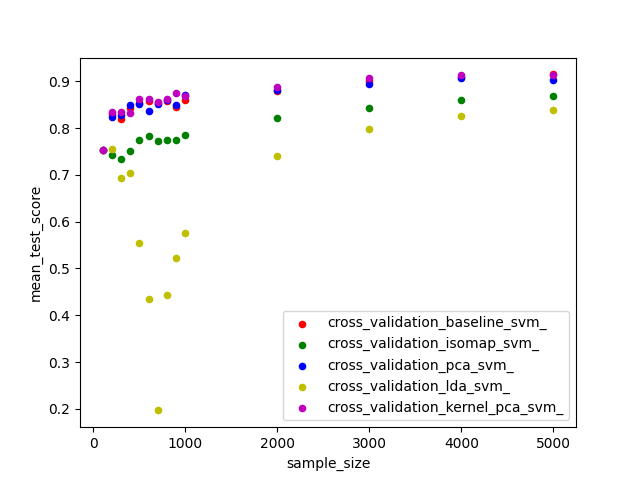
\includegraphics[width=0.8\textwidth]{figures/test_score_based_on_size.png}
    \caption{}
    \label{fig:experiment_4_performance_size}
\end{figure}


\begin{figure}[htb!]
    \centering
    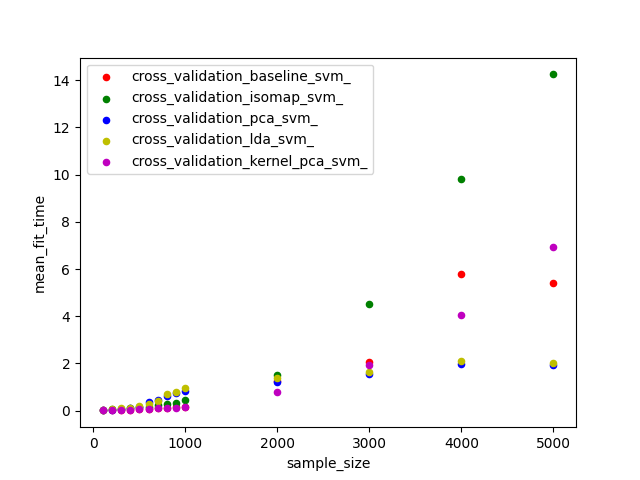
\includegraphics[width=0.8\textwidth]{figures/time_based_on_size.png}
    \caption{}
    \label{fig:experiment_4_speed_size}
\end{figure}


In terms of performance, \ref{fig:experiment_4_performance_size} shows that both baseline \gls{pca} and \gls{kpca} perform similarly well across all sample sizes, with consistently high F1 scores. In contrast, \gls{lda} performs worse overall, while \gls{isomap} has slightly lower F1 scores in smaller sample sizes but performs better in larger samples.

In terms of speed, \ref{fig:experiment_4_speed_size} shows that both \gls{pca} and \gls{lda} are the fastest when the sample size is larger than 2000, although they are slightly slower in smaller samples. Baseline \gls{pca} is the third slowest, while \gls{kpca} is the second slowest at a sample size of 5000. \gls{isomap} is the slowest overall, with longer runtimes for sample sizes of 2000 and above.

Overall, it appears that both \gls{pca} and \gls{kpca} are good choices for improving the performance of a \gls{svm} model on the \gls{mnist} data set, as they offer both high performance and fast runtime. \gls{lda} may be a less optimal choice due to its lower performance, while \gls{isomap} may be a bad option for larger sample sizes but may be suitable for smaller samples due to its slower runtime.


% The use of kernel principal component analysis  for dimensionality reduction may not have a significant impact on the performance of a support vector machine  model when applied to the \gls(mnist) data set. This is because the \gls(mnist) data set is already a low-dimensional data set, with only 784 features. In this case, using KPCA for dimensionality reduction may not provide much additional benefit, as the original data set is already well-suited for an SVM model. However, using KPCA may still have some advantages, such as the ability to remove noise and irrelevant information from the data set, and to visualize the data in a lower-dimensional space. Overall, while the use of KPCA with the \gls(mnist) data set may not have a major impact on the performance of the SVM model, it can still provide some benefits.